% XeLaTeX document
\documentclass[12pt,a4paper]{article}

% Редактируем: конфигурация, личные настройки: имя, название предмета и пр. для титульной страницы и метаданных документа здесь
\newcommand{\university}{Санкт-Петербургский политехнический университет Петра Великого}
\newcommand{\faculty}{Институт компьютерных наук и технологий}
\newcommand{\department}{Высшая школа интеллектуальный систем и суперкомпьютерных технологий}
\newcommand{\city}{Санкт-Петербург}
\newcommand{\docname}{Отчёт по лабораторным работам}
\newcommand{\subject}{Телекоммуникационные технологии}
\newcommand{\tutorname}{Н. В. Богач}
\newcommand{\studentname}{Е. К. Борисов}
\newcommand{\group}{3530901/90201}

% Не редактируем: используемые пакеты
% настройка кодировки, шрифтов и русского языка
\usepackage{fontspec}
\usepackage{polyglossia}

% рабочие ссылки в документе
\usepackage{hyperref}

% графика
\usepackage{graphicx}
\usepackage{tikz}

% поворот страницы
\usepackage{pdflscape}

% качественные листинги кода
\usepackage{minted}
\usepackage{listings}
\usepackage{lstfiracode}

% отключение копирования номеров строк из листинга, работает не во всех просмотрщиках (в Adobe Reader работает)
\usepackage{accsupp}
\newcommand\emptyaccsupp[1]{\BeginAccSupp{ActualText={}}#1\EndAccSupp{}}
\let\theHFancyVerbLine\theFancyVerbLine
\def\theFancyVerbLine{\rmfamily\tiny\emptyaccsupp{\arabic{FancyVerbLine}}}

% библиография
\bibliographystyle{templates/gost-numeric.bbx}
\usepackage{csquotes}
\usepackage[parentracker=true,backend=biber,hyperref=true,bibencoding=utf8,style=numeric-comp,language=auto,autolang=other,citestyle=gost-numeric,defernumbers=true,bibstyle=gost-numeric,sorting=ntvy]{biblatex}

% установка полей
\usepackage{geometry}

% нумерация картинок по секциям
\usepackage{chngcntr}

% дополнительные команды для таблиц
\usepackage{booktabs}

% для заголовков
\usepackage{caption}
\usepackage{titlesec}
\usepackage[dotinlabels]{titletoc}

% разное для математики
\usepackage{amsmath, amsfonts, amssymb, amsthm, mathtools}

% водяной знак на документе, см. main.tex
\usepackage[printwatermark]{xwatermark}

% Не редактируем: параметры используемых пакетов и не только
% настройки polyglossia
\setdefaultlanguage{russian}
\setotherlanguage{english}

% локализация
\addto\captionsrussian{
	\renewcommand{\figurename}{Рисунок}%
	\renewcommand{\partname}{Глава}
	\renewcommand{\contentsname}{\centerline{Содержание}}
	\renewcommand{\listingscaption}{Листинг}
}

% основной шрифт документа
\setmainfont{CMU Serif}
\newfontfamily\cyrillicfont{CMU Serif}[Script=Cyrillic]

% перечень использованных источников
\addbibresource{refs.bib}

% настройка полей
\geometry{top=2cm}
\geometry{bottom=2cm}
\geometry{left=2cm}
\geometry{right=2cm}
\geometry{bindingoffset=0cm}

% настройка ссылок и метаданных документа
\hypersetup{unicode=true,colorlinks=true,linkcolor=red,citecolor=green,filecolor=magenta,urlcolor=cyan,
	pdftitle={\docname},
	pdfauthor={\studentname},
	pdfsubject={\subject},
	pdfcreator={\studentname},
	pdfproducer={Overleaf},
	pdfkeywords={\subject}
}

% настройка подсветки кода и окружения для листингов
\usemintedstyle{colorful}
\newenvironment{code}{\captionsetup{type=listing}}{}

% шрифт для листингов с лигатурами
\setmonofont{FiraCode-Regular.otf}[
	SizeFeatures={Size=10},
	Path = templates/,
	Contextuals=Alternate
]

% оформления подписи рисунка
\captionsetup[figure]{labelsep = period}

% подпись таблицы
\DeclareCaptionFormat{hfillstart}{\hfill#1#2#3\par}
\captionsetup[table]{format=hfillstart,labelsep=newline,justification=centering,skip=-10pt,textfont=bf}

% путь к каталогу с рисунками
\graphicspath{{fig/}}

% Внесение titlepage в учёт счётчика страниц
\makeatletter
\renewenvironment{titlepage} {
	\thispagestyle{empty}
}
\makeatother

\counterwithin{figure}{section}
\counterwithin{table}{section}

\titlelabel{\thetitle.\quad}

% для удобного конспектирования математики
\mathtoolsset{showonlyrefs=true}
\theoremstyle{plain}
\newtheorem{theorem}{Теорема}[section]
\newtheorem{proposition}[theorem]{Утверждение}
\theoremstyle{definition}
\newtheorem{corollary}{Следствие}[theorem]
\newtheorem{problem}{Задача}[section]
\theoremstyle{remark}
\newtheorem*{nonum}{Решение}

% настоящее матожидание
\newcommand{\MExpect}{\mathsf{M}}

% объявили оператор!
\DeclareMathOperator{\sgn}{\mathop{sgn}}

% перенос знаков в формулах (по Львовскому)
\newcommand*{\hm}[1]{#1\nobreak\discretionary{} {\hbox{$\mathsurround=0pt #1$}}{}}


% водяной знак для обозначения статуса документа
% \newwatermark[allpages,color=red!5,angle=45,scale=3,xpos=0,ypos=0]{DRAFT}
\begin{document}
% Не редактируем: Титульная страница (формируется автоматически из заданной конфигурации)
\begin{titlepage}	% начало титульной страницы

	\begin{center}		% выравнивание по центру

		\large \university \\
		\large \faculty \\
		\large \department \\[6cm]
		% название института, затем отступ 6см

		\huge \subject \\[0.5cm] % название работы, затем отступ 0,5см
		\large \docname \num \\[5.1cm]
		% \large Тема работы\\[5cm]

	\end{center}


	\begin{flushright} % выравнивание по правому краю
		\begin{minipage}{0.25\textwidth} % врезка в половину ширины текста
			\begin{flushleft} % выровнять её содержимое по левому краю

				\large\textbf{Работу выполнил:}\\
				\large \studentname \\
				\large {Группа:} \group \\

				\large \textbf{Преподаватель:}\\
				\large \tutorname

			\end{flushleft}
		\end{minipage}
	\end{flushright}

	\vfill % заполнить всё доступное ниже пространство

	\begin{center}
		\large \city \\
		\large \the\year % вывести дату
	\end{center} % закончить выравнивание по центру

\end{titlepage} % конец титульной страницы

\vfill % заполнить всё доступное ниже пространство


% Не редактируем: Страница содержания (формируется автоматически из section, subsection и пр., указанных в content.tex)
% Содержание
\tableofcontents
\newpage



% Редактируем: всё остальное: вступление, др. этапы, заключение, приложение
\section{Звуки и сигналы}
\subsection{Упражнение 1}

Скачайте с сайта http://freesound.org , включающий музыку, речь или иные звуки, имеющие четко выраженную высоту. Выделите примерно полусекундный сегмент, в котором высота постоянна. Вычислите и распечатайте спектр выбранного сегмента. Как связаны тембр звука и гармоническая структура, видимая в спектре?


\noindent Используйте high\_pass, low\_pass, и band\_stop для фильтрациитех или иных гармоник. Затем преобразуйте спектры обратно в сигнал и прослушайте его. Как звук соотносится с изменениями, сделанными в спектре?
    

Был выбран звук пианино, загружаем его, прослушиваем, затем вырезаем полусекундный фрагмент выбранного звука и строим wave график.

\begin{lstlisting}[language=Python]
if not os.path.exists('440931__xhale303__piano-loop-1.wav'):
    !wget https://github.com/Eugenepolyt/ThinkDSP/raw/master/440931__xhale303__piano-loop-1.wav
wave = read_wave('440931__xhale303__piano-loop-1.wav')
wave.make_audio()
segment = wave.segment(start=1.5, duration=0.5)
segment.make_audio()
segment.plot()
\end{lstlisting}
    
\begin{figure}[H]
	\begin{center}
		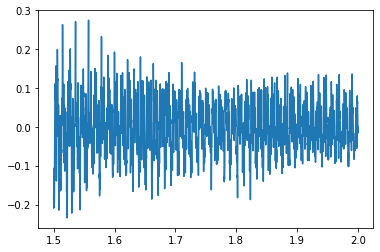
\includegraphics[scale=1]{fig/lab01/lab01_1.png}
		\caption{График выделенного сегмента}
	\end{center}
\end{figure}

Вычислим спектр выделенного сегмента и построим график.
\begin{lstlisting}[language=Python]
spectrum = segment.make_spectrum()
spectrum.plot(high=3000)
decorate(xlabel='Frequency')
\end{lstlisting}

\begin{figure}[H]
	\begin{center}
		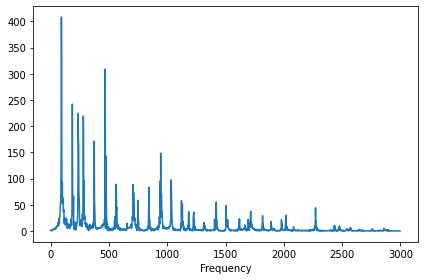
\includegraphics[scale=1]{fig/lab01/lab01_2.png}
		\caption{Спектр звука фрагмента}
	\end{center}
\end{figure}

В данном примере основная частота является доминирующей, воспринимаемая высота звука сильно зависит от основной частоты. Используем функции для фильтрации для данного спектра.


Уберем частоты выше 1500.

\begin{lstlisting}[language=Python]
spectrum.low_pass(1500)
spectrum.plot(high=3000)
decorate(xlabel='Frequency')
\end{lstlisting}

\begin{figure}[H]
	\begin{center}
		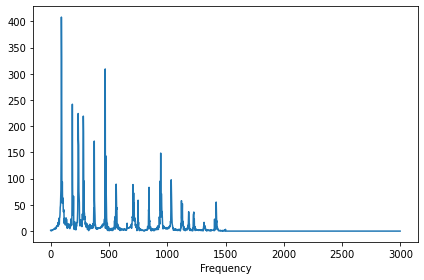
\includegraphics[scale=1]{fig/lab01/lab01_3.png}
		\caption{Спектр звука c урезанными частотами}
	\end{center}
\end{figure}

Уберем частоты ниже 400, тем самым изменим доминирующую частоту.

\begin{figure}[H]
	\begin{center}
		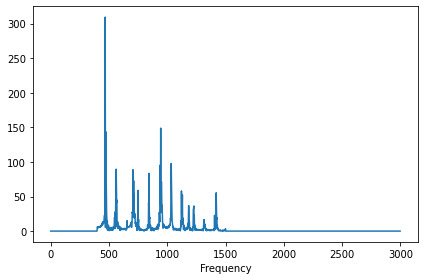
\includegraphics[scale=1]{fig/lab01/lab01_4.png}
		\caption{Спектр звука c частотами выше 400 и ниже 1500}
	\end{center}
\end{figure}

Применим ФПЗ.

\begin{lstlisting}[language=Python]
spectrum.band_stop(500, 800)
spectrum.plot(high=3000)
decorate(xlabel='Frequency')
\end{lstlisting}

\begin{figure}[H]
	\begin{center}
		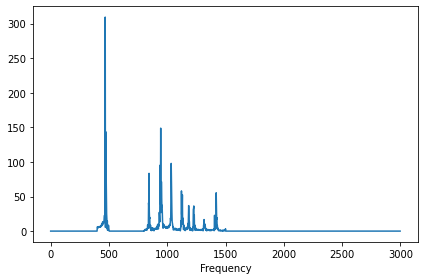
\includegraphics[scale=1]{fig/lab01/lab01_5.png}
		\caption{Спектр звука после ФПЗ}
	\end{center}
\end{figure}

Преобразуем спектр обратно в сигнал.

\begin{lstlisting}[language=Python]
filtered = spectrum.make_wave()
filtered.plot()
decorate(xlabel='Time')
\end{lstlisting}

Сравниваем первоначальный сигнал с отфильтрованным фрагментом.

\begin{lstlisting}[language=Python]
segment.make_audio()
filtered.make_audio()
\end{lstlisting}

После обработки звук звучит уже не так объемно, и напоминает гудок, а не пианино

\subsection{Упражнение 2}

Создайте сложный сигнал из объектов SinSignal и CosSignal, суммируя их. Обработайте сигнал для получения wave и прослушайте его. Вычислите Spectrum и распечатайте. Что произойдёт при добавлении частотных компонент, не кратных основным?


Создадим сложный сигнал из CosSignal и SinSignal и построим график.
\begin{lstlisting}[language=Python]
cos_sig = CosSignal(freq=50, amp=0.8, offset=0)
sin_sig = SinSignal(freq=200, amp=0.4, offset=0)
cos2_sig = SinSignal(freq=600, amp=0.6, offset=0)
sin2_sig = SinSignal(freq=1000, amp=0.2, offset=0)
m_sig = cos_sig + sin_sig + sin2_sig + cos2_sig
\end{lstlisting}

\begin{figure}[H]
	\begin{center}
		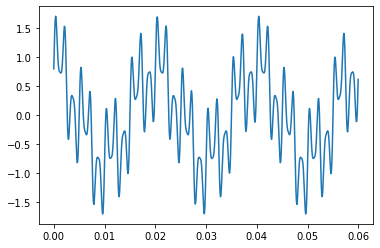
\includegraphics[scale=1]{fig/lab01/lab01_6.png}
		\caption{Граффик после суммирования сигналов}
	\end{center}
\end{figure}

Создадим wave и вычислим спектр.

\begin{lstlisting}[language=Python]
wave = m_sig.make_wave()
wave.make_audio()
spectrum = wave.make_spectrum()
spectrum.plot()
\end{lstlisting}

\begin{figure}[H]
	\begin{center}
		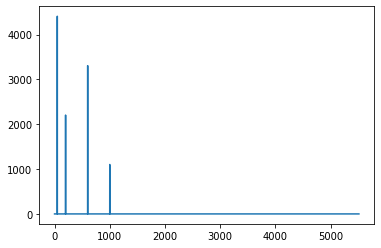
\includegraphics[scale=1]{fig/lab01/lab01_7.png}
		\caption{Спектр сигнала}
	\end{center}
\end{figure}

Добавим частотный компонент, не кратный основным.

\begin{lstlisting}[language=Python]
secondWave = (m_sig + CosSignal(freq=440, amp=0.75, offset=0)).make_wave()
secondWave.make_audio()
spectr = secondWave.make_spectrum()
spectr.plot()
\end{lstlisting}

\begin{figure}[H]
	\begin{center}
		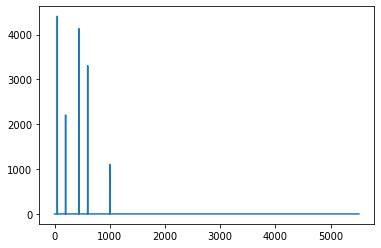
\includegraphics[scale=1]{fig/lab01/lab01_8.png}
		\caption{Спектр после изменения}
	\end{center}
\end{figure}

После изменения звук стал не таким однотонным, каким был. 


\subsection{Упражнение 3}

Напишите функцию strech, берущую wave и коэффицент изменения. Она должна ускорять или замедлять сигнал изменением ts и framerate.

Напишем необходимую функцию.

\begin{lstlisting}[language=Python]
def stretch(wave, coef):
  wave.ts *= coef
  wave.framerate /= coef
\end{lstlisting}

\begin{figure}[H]
	\begin{center}
		
\includegraphics[scale=1]{fig/lab01/lab01_9.png}
		\caption{Длинна изначального звука пианино}
	\end{center}
\end{figure}

Попробуем ускорить и замедлить звук пианино.

\begin{lstlisting}[language=Python]
fasterX2 = wave
stretch(fasterX2, 0.5)
fasterX2.make_audio()

slowX2 = read_wave('440931__xhale303__piano-loop-1.wav')
stretch(slowX2, 2)
slowX2.make_audio()
\end{lstlisting}

\begin{figure}[H]
	\begin{center}
		
\includegraphics[scale=1]{fig/lab01/lab01_10.png}
		\caption{Длинна ускоренного звука}
	\end{center}
\end{figure}

\begin{figure}[H]
	\begin{center}
		
\includegraphics[scale=1]{fig/lab01/lab01_11.png}
		\caption{Длинна замедленного звука}
	\end{center}
\end{figure}

По рисункам можно заметить , что функция работает весьма успешно, в случае ускорения длинна дорожки сокращается в два раза, в случае замедленния, увеличивается в два раза.



\subsection{Вывод}
В данной лабораторной работе, были изучены основные понятия при работе со звуком и проведена работа с библиотекой thinkDSP, которая позваляет производить различные действия с сигналами.
\newpage

\section{Гармоники}
\subsection{Упражнение 1}

Пилообразный сигнал линейно нарастает от -1 до 1, а затем резко падает до -1 и повторяется.

\noindent Напишите класс, называемый SawtoothSignal, расширяющий signal и предоставляющий evaluate для оценки пилообразного сигнала.

\noindent Вычислите спектр пилообразного сигнала. Как соотносится его гармоническая структура с тругольными с прямоугольными сигналами?

Для создания пилообразного сигнала создадим класс SawtoothSignal. В методе класса evaluate опишем число циклов и c помощью библиотеки numpy разделим число циклов. unbias - смещает сигнал а normalize масштабирует его до заданной амплитуды.

\begin{lstlisting}[language=Python]
import thinkdsp

class SawtoothSignal(thinkdsp.Sinusoid):
  def evaluate(self, ts):
    cycles = self.freq * ts + self.offset / np.pi / 2
    frac, _ = np.modf(cycles)
    ys = thinkdsp.normalize(thinkdsp.unbias(frac), self.amp)
    return ys
\end{lstlisting}

\noindent Отобразим график пилообразного сигнала.

\begin{lstlisting}[language=Python]
saw = SawtoothSignal()
saw.plot()
saw_wave = saw.make_wave(duration=3, framerate=10000)
\end{lstlisting}

\begin{figure}[H]
	\begin{center}
		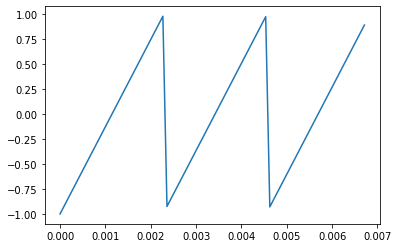
\includegraphics[scale=1]{fig/lab02/lab02_1.png}
		\caption{График пилообразного сигнала}
	\end{center}
\end{figure}

Вычислим спектр.

\begin{lstlisting}[language=Python]
spectr = saw_wave.make_spectrum()
spectr.plot()
\end{lstlisting}

\begin{figure}[H]
	\begin{center}
		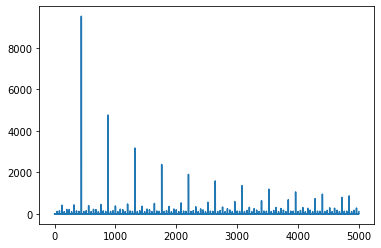
\includegraphics[scale=1]{fig/lab02/lab02_2.png}
		\caption{Спектр пилообразного сигнала}
	\end{center}
\end{figure}

Теперь сравним полученный спектр с треугольными и прямоугольными сигналами.

\begin{lstlisting}[language=Python]
triangle = TriangleSignal()
triangle.make_wave(duration=3, framerate=10000).make_spectrum().plot()
\end{lstlisting}

\begin{figure}[H]
	\begin{center}
		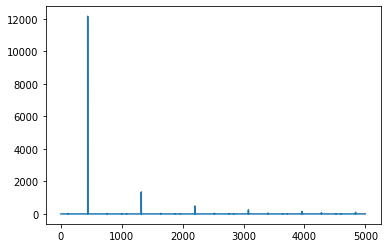
\includegraphics[scale=1]{fig/lab02/lab02_3.png}
		\caption{Спектр треугольного сигнала}
	\end{center}
\end{figure}

\begin{lstlisting}[language=Python]
square = SquareSignal()
square.make_wave(duration=3, framerate=10000).make_spectrum().plot()
\end{lstlisting}

\begin{figure}[H]
	\begin{center}
		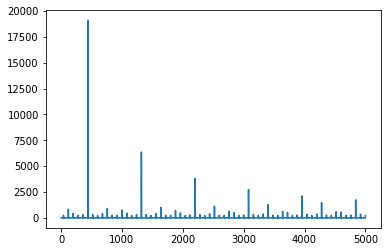
\includegraphics[scale=1]{fig/lab02/lab02_4.png}
		\caption{Спектр прямоугольного сигнала}
	\end{center}
\end{figure}

Можно заметить, в сравнении с треугольным сигналом, его амплитуда падает пропорцианально квадрату частоты, а у пилообразного пропорцианально частоте, ровно также как и у квадратного сигнала, однако пилообразный включает в себя как четные, так и нечетные гармоники, когда у квадратного только нечетные.

\subsection{Упражнение 2}

Создайте прямугольный сигнал 1100 Гц и вычислите wave с выборками 10 000 кадров в секунду. Постройте спектр и убедитесь, что большинство гармоник "завёрнуты" из-за биений, слышно ли последствия этого при проигрывании?

\begin{lstlisting}[language=Python]
square = thinkdsp.SquareSignal(1100)
segment = square.make_wave(duration=1, framerate=10000)
spectr = segment.make_spectrum()
spectr.plot()
\end{lstlisting}

\begin{figure}[H]
	\begin{center}
		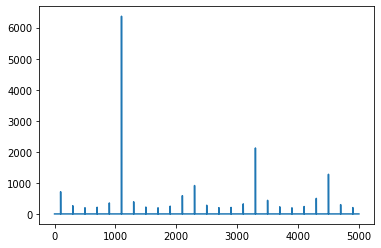
\includegraphics[scale=1]{fig/lab02/lab02_5.png}
		\caption{Спектр сигнала с биениями}
	\end{center}
\end{figure}

На спектре видно, что происходит "завернутость" биений, гармоники 1100 и 3300 выстроены верно, однако видно, что третий и четвертый пик находятся на 4500 и 2300 соответственно, они неотличимы от 5500 и 7700


\subsection{Упражнение 3}

Возьмите объект спектра spectrum, и выведите первые несколько значений spectrum.fs, вы увидите, что частоты начинаются с нуля. Итак, «spectrum.hs[0]» — это величина компонента с частотой 0. Но что это значит?

\noindent Попробуйте этот эксперимент:

1. Сделать треугольный сигнал с частотой 440 и создать Волну длительностью 0,01 секунды. Постройте форму волны.

2. Создайте объект Spectrum и напечатайте spectrum.hs[0]. Каковы амплитуда и фаза этой составляющей?

3. Установите spectrum.hs[0] = 100. Создайте волну из модифицированного спектра и выведите ее. Как эта операция влияет на форму сигнала?

Создадим треугольный сигнал с частотой 440Hz и длительностью 0,01 сек, построим его график, распечатаем сигнал и распечатаем Spectrum.hs[0].


\begin{lstlisting}[language=Python]
signal = thinkdsp.TriangleSignal(440)
segment = signal.make_wave(0.01, framerate=10000)
segment.plot()
\end{lstlisting}

\begin{figure}[H]
	\begin{center}
		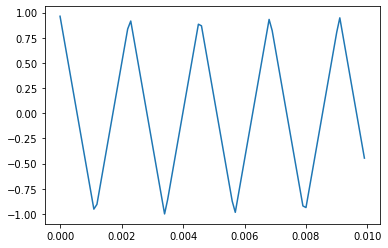
\includegraphics[scale=1]{fig/lab02/lab02_6.png}
		\caption{График сигнала}
	\end{center}
\end{figure}

Проверим что лежит в 0 элементе.

\begin{lstlisting}[language=Python]
spectr = segment.make_spectrum()
spectr.hs[0]
\end{lstlisting}

\begin{lstlisting}
(3.375077994860476e-14+0j)
\end{lstlisting}
Каждый элмент массива hs объекта Spectrum представялет собой комплексное число. Они соотвествуют частотной компоненте: размах пропоцианален амплитуде соответствующей компоненты, а угол - это фаза.

\noindent Видно, что первый элемент массива hs - это комплексное число близкое к нулю. Установим этому элементу значение 100 и посмотрим на результат
\begin{lstlisting}[language=Python]
spectr.hs[0] = 100
spectr.make_wave().plot()
\end{lstlisting}

\begin{figure}[H]
	\begin{center}
		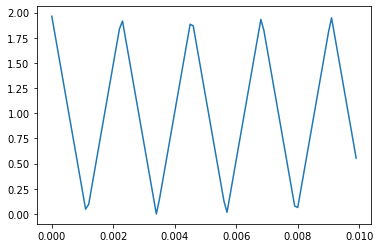
\includegraphics[scale=1]{fig/lab02/lab02_7.png}
		\caption{График сигнала с изменённым нулевым числом спекторграммы}
	\end{center}
\end{figure}

Из полученного графика видно смещение сигнала по вертикали, таким образом можно сделать вывод о том, что первый элемент отвечает за смещение по вертикали, в случае, если он близок к нулю, то сигнал не смещается.

\subsection{Упражнение 4}

Напишите функцию, которая принимает Spectrum в качестве параметра и модифицирует его, деля каждый элемент hs на соответствующую частоту из fs. Протестируйте свою функцию, используя один из файлов WAV в репозитории или любой объект Wave.

1. Рассчитайте спектр и начертите его.

2. Измените спектр, используя свою функцию, и снова начертите его.

3. Сделать волну из модифицированного Spectrum и прослушать ее. Как эта операция влияет на сигнал?


Напишем функцию которая принимает на вход Spectrum и изменяет его его делением каждого элемента hs на соответствующую частоту fs и проверим эту функцию на треугольном сигнале

\begin{lstlisting}[language=Python]
def spec_div(spec):
  spec.hs[1:] /= spec.fs[1:]
  spec.hs[0] = 0
  spec.plot()

triangle = TriangleSignal()
wave = triangle.make_wave(duration=0.5, framerate=10000)
wave.make_audio()

spectr = wave.make_spectrum()
spectr.plot()
\end{lstlisting}

\begin{figure}[H]
	\begin{center}
		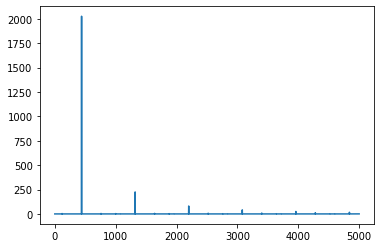
\includegraphics[scale=1]{fig/lab02/lab02_8.png}
		\caption{Спектр треугольного сигнала}
	\end{center}
\end{figure}

Применим написанную функцию.

\begin{lstlisting}[language=Python]
spec_div(spectr)
\end{lstlisting}

\begin{figure}[H]
	\begin{center}
		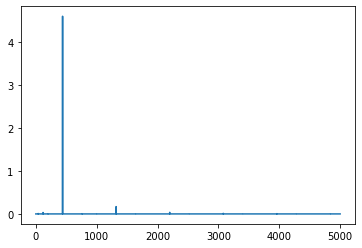
\includegraphics[scale=1]{fig/lab02/lab02_9.png}
		\caption{Спектр изменённого сигнала}
	\end{center}
\end{figure}

\begin{lstlisting}[language=Python]
spectr.make_wave().make_audio()
\end{lstlisting}

Если прослушать полученный звук, можно услышать что он стал тише и чище, это связано с работой функции, которая ослабляет низкие частоты на некоторую величину.

\subsection{Упражнение 5}

Треугольные и прямоугольные волны имеют только нечетные гармоники; пилообразная волна имеет как четные, так и нечетные гармоники. Гармоники прямоугольной и пилообразной волн затухают пропорционально $1/f$; гармоники треугольной волны затухают как $1/f^2$. Можете ли вы найти форму волны, в которой четные и нечетные гармоники затухают как $1/f^2$?

\noindent Подсказка: есть два способа подойти к этому: вы можете построить нужный сигнал путем сложения синусоид, или вы может начаться с сигнала, похожего на то, что вы хотите, и изменить его.


\noindent Создадим сигнал, состоящий из четных и нечетных гармоник, при этом, чтобы они падали пропорцианально квадрату частоты. Возьмем пилообразный сигнал, который имет четные и нечетные гармоники, а далее скорректируем его спад при помощи функции из предыдущего упражнения.

\begin{lstlisting}[language=Python]
saw_sign = SawtoothSignal(400)
saw_w = saw_sign.make_wave(duration=0.5, framerate=20000)
spectr = saw_w.make_spectrum()
spectr.plot()
decorate(xlabel='Frequency (Hz)')
\end{lstlisting}

\begin{figure}[H]
	\begin{center}
		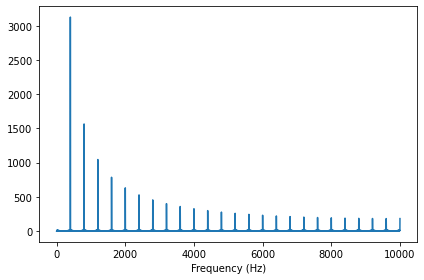
\includegraphics[scale=1]{fig/lab02/lab02_10.png}
		\caption{Спектр пилообразного сигнала}
	\end{center}
\end{figure}

Применим функцию для изменения амплитуды спада

\begin{lstlisting}[language=Python]
spec_div(spectr)
spectr.scale(400)
spectr.plot()
\end{lstlisting}

\begin{figure}[H]
	\begin{center}
		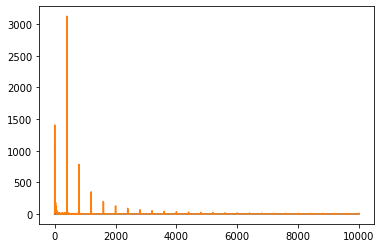
\includegraphics[scale=1]{fig/lab02/lab02_11.png}
		\caption{Спектр пилообразного сигнала после функции}
	\end{center}
\end{figure}

\begin{lstlisting}[language=Python]
spectr.make_wave().segment(duration=0.01).plot()
\end{lstlisting}

\begin{figure}[H]
	\begin{center}
		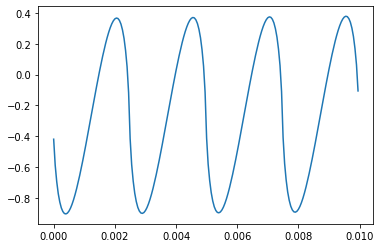
\includegraphics[scale=1]{fig/lab02/lab02_12.png}
		\caption{График сигнала}
	\end{center}
\end{figure}

Видно, что спектр спадает пропорционально квадрату частоты и при этом имеет четные и нечетные гармоники

\subsection{Вывод}

В данной работе были произведены различные действия с разными видами сигналов, были рассмотрены спектры и гармонические структуры и биения.
\newpage

\section{Непериодические сигналы}
\subsection{Упражнение 1}

Запустите и прослушайте примеры в файле chap03.ipynb. В примере с утечкой попробуйте заменить окно Хэмминга одним из других окон, предоставляемых NumPy, и посмотрите, как они влияют на утечку.

\begin{lstlisting}[language=Python]
signal = SinSignal(freq=440)
duration = signal.period * 30.25
wave = signal.make_wave(duration)
spectrum = wave.make_spectrum()
spectrum.plot(high=880)
\end{lstlisting}

\begin{figure}[H]
	\begin{center}
		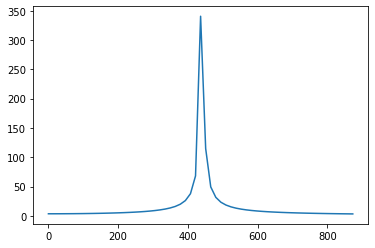
\includegraphics[scale=1]{fig/lab03/lab03_1.png}
		\caption{Рассматриваемый сигнал}
	\end{center}
\end{figure}

Посмотрим как выглядит спектограмма с использованием окна Хэмминга:

\begin{figure}[H]
	\begin{center}
		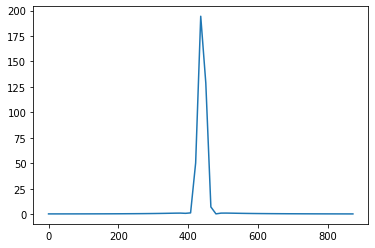
\includegraphics[scale=1]{fig/lab03/lab03_2.png}
		\caption{Сигнал с использованием окна Хэмминга}
	\end{center}
\end{figure}


Используем другое окно а именно Барлетта

\begin{lstlisting}[language=Python]
wave = signal.make_wave(duration)
wave.ys *= np.bartlett(len(wave.ys))
spectrum = wave.make_spectrum()
spectrum.plot(high=880)
\end{lstlisting}
\begin{figure}[H]
	\begin{center}
		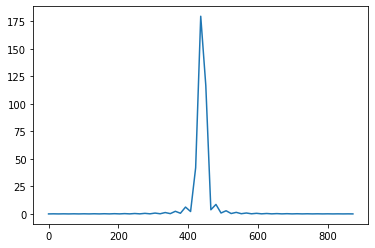
\includegraphics[scale=1]{fig/lab03/lab03_3.png}
		\caption{Сигнал с использованием окна Барлетта}
	\end{center}
\end{figure}

Можно заметить. что низкие амплитуды стали ломанными линиями.

\subsection{Упражнение 2}


Напишите класс SawtoothChirp, расширяющий Chirp и переопределяющий evaluate для генерации пилообразного сигнала с линейно увеличивающейся частотой.

\begin{lstlisting}[language=Python]
import thinkdsp
from thinkdsp import normalize, unbias
from math import pi

class SawtoothChirp(Chirp):

    def evaluate(self, ts):
        freqs = np.linspace(self.start, self.end, len(ts))
        dts = np.diff(ts, prepend=0)
        dphis = (2 * np.pi) * freqs * dts
        phases = np.cumsum(dphis)
        cycles = phases / (2 * np.pi)
        frac, _ = np.modf(cycles)
        ys =  normalize(unbias(frac), self.amp)
        return ys
\end{lstlisting}

Создадим пилообразный сигнал от второй до пятой октавы "ля" 880 - 7040.

\begin{lstlisting}[language=Python]
signal = SawtoothChirp(start=880, end=7040)
wave = signal.make_wave(duration=3, framerate=4000)
wave.apodize()
wave.make_audio()
sp = wave.make_spectrogram(seg_length=512)
sp.plot(high=5000)
\end{lstlisting}

\begin{figure}[H]
	\begin{center}
		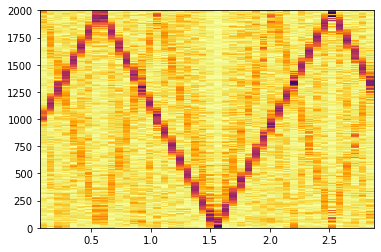
\includegraphics[scale=1]{fig/lab03/lab03_4.png}
		\caption{Спектр сигнала}
	\end{center}
\end{figure}

По звуку и эскизу виден эффект биения.


\subsection{Упражнение 3}

Создайте пилообразный чирп, меняющийся от 2500 до 3000 Гц, и на его основе сгенерируйте сигнал длительностью 1 с и частотой кадоров 20 кГц. Нарисуйте, каким примерно будет Spectrum. Затем распечатайте Spectrum и посмотрите, правы ли вы.

\begin{lstlisting}[language=Python]
sawC = SawtoothChirp(start=2500, end=3000)
wave = sawC.make_wave(duration=1, framerate=20000)
wave.make_spectrum().plot()
\end{lstlisting}
\begin{figure}[H]
	\begin{center}
		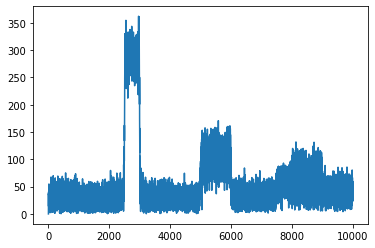
\includegraphics[scale=1]{fig/lab03/lab03_5.png}
		\caption{Спектр сигнала}
	\end{center}
\end{figure}

По графику видно, что ожидаемо базовая частота находится в пределах от 2500Hz до 3500 Hz, следующие же гармоники отличаются от базовой и находятся на частотах от 5000 до 6000 и 7500 до 9000 герц, остальные гармоники наложены друг на друга

\subsection{Упражнение 4}

В музыкальной терминологии «глиссандо» — это нота, которая скользит от одной высоты тона к другой, поэтому она похожа на чириканье. Найдите или сделайте запись глиссандо и постройте его спектрограмму.

Для вывода соответствующей спектограммы, возьмем нужный нам звук из репозитория учебника:

\begin{lstlisting}[language=Python]
if not os.path.exists('72475__rockwehrmann__glissup02.wav'):
    !wget https://github.com/AllenDowney/ThinkDSP/raw/master/code/72475__rockwehrmann__glissup02.wav
    
from thinkdsp import read_wave
wave = read_wave('72475__rockwehrmann__glissup02.wav')
wave.make_audio()
wave.make_spectrogram(512).plot(high=5000)
\end{lstlisting}
\begin{figure}[H]
	\begin{center}
		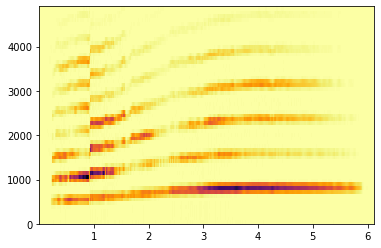
\includegraphics[scale=1]{fig/lab03/lab03_6.png}
		\caption{Спектрограмма сигнала}
	\end{center}
\end{figure}

Видим, что спектограмма очень похожа на наш чирп.

\subsection{Упражнение 5}

Тромбонист может играть глиссандо, выдвигая слайд тромбона и непрерывно дуя. По мере выдвижения ползуна общая длина трубки увеличивается, а результирующий шаг обратно пропорционален длине.
Предполагая, что игрок перемещает слайд с постоянной скоростью, как меняется ли частота со временем?

\noindent Напишите класс TromboneGliss, расширяющий класс Chirp и предоставляет evaluate. Создайте волну, имитирующую тромбон глиссандо от F3 вниз до C3 и обратно до F3. C3 — 262 Гц; F3 есть 349 Гц.

\begin{lstlisting}[language=Python]
class TromboneGliss(Chirp): 
    def evaluate(self, ts):
        lengths = np.linspace(1.0 / self.start, 1.0 / self.end, len(ts))
        freqs = 1 / lengths
        dts = np.diff(ts, prepend=0)
        dphis = np.pi * 2 * freqs * dts
        phases = np.cumsum(dphis)
        ys = self.amp * np.cos(phases)
        return ys
\end{lstlisting}

Создадим два сигнала-глиссандо от С3 до F3 и от F3 к C3 и соеденим эти два сигнала.

\begin{lstlisting}[language=Python]
firstSignal = TromboneGliss(262, 349)
firstWave = firstSignal.make_wave(duration=1)
spectr = firstWave.make_spectrogram(1024)
spectr.plot(high=1000)
\end{lstlisting}
\begin{figure}[H]
	\begin{center}
		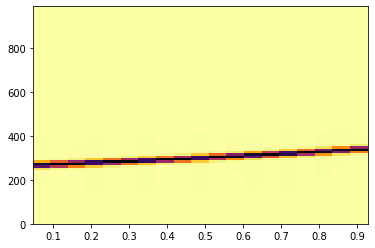
\includegraphics[scale=1]{fig/lab03/lab03_7.png}
		\caption{Спектрограмма первого сигнала}
	\end{center}
\end{figure}

\begin{lstlisting}[language=Python]
secondSignal = TromboneGliss(349, 262)
secondWave = secondSignal.make_wave(duration=1)
secondWave.make_audio()
spectr = secondWave.make_spectrogram(1024)
spectr.plot(high=1000)
\end{lstlisting}

\begin{figure}[H]
	\begin{center}
		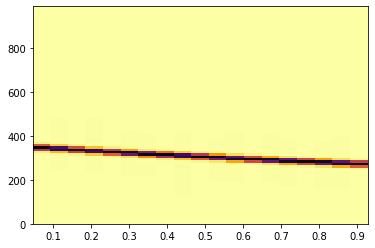
\includegraphics[scale=1]{fig/lab03/lab03_8.png}
		\caption{Спектрограмма второго сигнала}
	\end{center}
\end{figure}

Объеденим сигналы

\begin{lstlisting}[language=Python]
result = firstWave | secondWave
result.make_audio()
spectr = result.make_spectrogram(1024)
spectr.plot(high=1000)
\end{lstlisting}

\begin{figure}[H]
	\begin{center}
		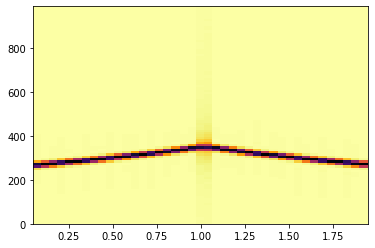
\includegraphics[scale=1]{fig/lab03/lab03_9.png}
		\caption{Спектрограмма объедененного сигнала}
	\end{center}
\end{figure}

Слышно, как две части идут друг за другом, также это хорошо видно на графике

\subsection{Упражнение 6}

Сделайте или найдите запись серии гласных звуков и посмотрите на спектрограмму. Сможете ли вы различить разные гласные?

Снова воспользуемся репозиторием учебника и возьмем оттуда звуки глассных.

\begin{lstlisting}[language=Python]
if not os.path.exists('87778__marcgascon7__vocals.wav'):
    !wget https://github.com/AllenDowney/ThinkDSP/raw/master/code/87778__marcgascon7__vocals.wav
wave = read_wave('87778__marcgascon7__vocals.wav')
wave.make_audio()
wave.make_spectrogram(1024).plot(1000)
\end{lstlisting}
\begin{figure}[H]
	\begin{center}
		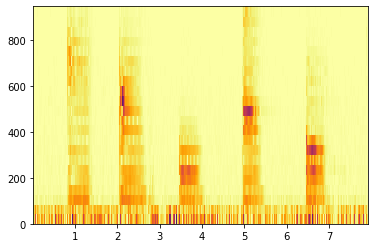
\includegraphics[scale=1]{fig/lab03/lab03_10.png}
		\caption{Спектрограмма гласных звуков}
	\end{center}
\end{figure}

На записи глассных есть 5 звуков и по спектограмме отчетливо видны эти глассные звуки в виде пиков.

\subsection{Вывод}

В данной работе были рассмотрены частотные компоненты и апериодические сигналы.

\newpage

\section{Шумы}
\subsection{Упражнение 1}

«A Soft Murmur» — это веб-сайт, на котором можно послушать множество естественных источников шума, включая дождь, волны, ветер и т. д. 

\noindent На http://asoftmurmur.com/about/ вы можете найти их список записей, большинство из которых находится на http://freesound.org.

\noindent Загрузите несколько таких файлов и вычислите спектр каждого сигнала. Спектр мощности похож на белый шум, розовый шум, или броуновский шум? Как изменяется спектр во времени?

Возьмем звук моря и выделим два сегмента.

\begin{lstlisting}[language=Python]
if not os.path.exists('13793__soarer__north-sea.wav'):
    !wget https://github.com/Eugenepolyt/telecomunaction/raw/main/13793__soarer__north-sea.wav
from thinkdsp import read_wave
wave = read_wave('13793__soarer__north-sea.wav')
wave.make_audio()
segment = wave.segment(start=15, duration=1.0)
segment.make_audio()
segment.plot()
\end{lstlisting}
\begin{figure}[H]
	\begin{center}
		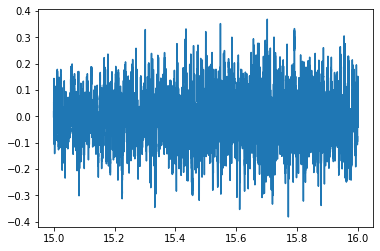
\includegraphics[scale=1]{fig/lab04/lab04_1.png}
		\caption{График сигнала}
	\end{center}
\end{figure}

Определим характеристики шума.

\begin{lstlisting}[language=Python]
from thinkdsp import decorate
spectrum.plot_power()

loglog = dict(xscale='log', yscale='log')
decorate(xlabel='Frequency (Hz)',
         ylabel='Power', 
         **loglog)
\end{lstlisting}
\begin{figure}[H]
	\begin{center}
		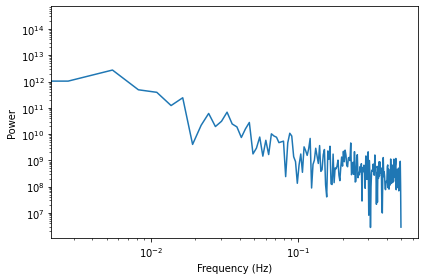
\includegraphics[scale=1]{fig/lab04/lab04_2.png}
		\caption{Спектр в логорифмическом масштабе}
	\end{center}
\end{figure}

График напоминает белый шум, возьмем теперь идущий за ним другой сегмент.

\begin{lstlisting}[language=Python]
segmentNext = wave.segment(start=16, duration=1.0)
segmentNext.make_audio()

spectrumNext = segmentNext.make_spectrum()
spectrum.plot_power()
spectrumNext.plot_power()

loglog = dict(xscale='log', yscale='log')
decorate(xlabel='Frequency (Hz)',
         ylabel='Power', 
         **loglog)
\end{lstlisting}
\begin{figure}[H]
	\begin{center}
		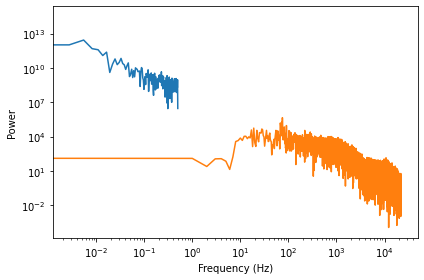
\includegraphics[scale=1]{fig/lab04/lab04_3.png}
		\caption{Сравнение спектров в логорифмическом масштабе}
	\end{center}
\end{figure}


\subsection{Упражнение 2}

Реализуйте метод Бартлетта\cite{barlett} и используйте его для оценки спектра мощности шумового сигнала. Подсказка: посмотрите на реализацую make\_spectrogram.

Реализуем метод Бартлетта для оценки спектра мощности шумового сигнала. Данный метод будет разделять сигнал на сегменты, вычислять для них разложение Фурье, вычислять сумму квадратов, находить среднее и вычислять корень.


\begin{lstlisting}[language=Python]
from thinkdsp import Spectrum

def make_barlett(wave, N, flag=True):
  spectrogram = wave.make_spectrogram(N,flag)
  spec_mac = spectrogram.spec_map.values()

  powers = []
  for spectrum in spec_mac:
    powers.append(spectrum.power)
  
  hs = np.sqrt(sum(powers)/ len(powers))
  fs = next(iter(spec_mac)).fs

  return Spectrum(hs, fs, wave.framerate)
\end{lstlisting}

Проведем тестирование на сигнале с предыдущего задания.

\begin{lstlisting}[language=Python]
barlett = make_barlett(segmentNext,1024)
barlett.plot_power()
decorate(xlabel='Frequency (Hz)', 
         ylabel='Power', 
         **loglog)
\end{lstlisting}

\begin{figure}[H]
	\begin{center}
		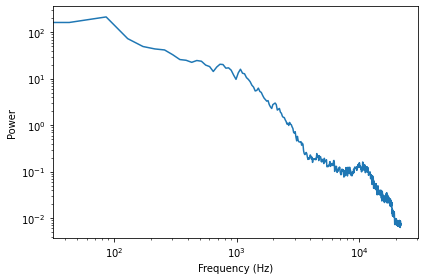
\includegraphics[scale=1]{fig/lab04/lab04_4.png}
		\caption{Результат работы функции}
	\end{center}
\end{figure}


\subsection{Упражнение 3}

Загрузите в виде CSV-файла исторические данные о ежедневной цене BitCoin. Откройте этот файл и вычислите спектр цен BitCoin как функцию времени. Похоже ли это на белый, розовый или броуновский шум?

Скачаем csv файл с ценами на биткоин

\begin{lstlisting}[language=Python]
if not os.path.exists('market-price.csv'):
    !wget https://github.com/Eugenepolyt/telecomunaction/raw/main/market-price.csv
import csv
worth = []
with open('market-price.csv') as File:
  reader = csv.reader(File, delimiter=',', quotechar=',',
                        quoting=csv.QUOTE_MINIMAL)
  for row in reader:
    worth.append(row[1])
worth = worth [1:]
days = a=np.arange(0,len(worth))
\end{lstlisting}
\begin{lstlisting}[language=Python]
from thinkdsp import Wave
wave = Wave(worth,days,1)
spectrum = wave.make_spectrum()
spectrum.plot_power()
decorate(xlabel='Частота',
         ylabel='Мощность', 
         **loglog)
\end{lstlisting}

\begin{figure}[H]
	\begin{center}
		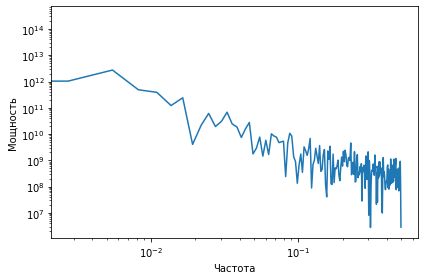
\includegraphics[scale=1]{fig/lab04/lab04_5.png}
		\caption{Спектрограмма цен BitCoin в логорифмическом формате}
	\end{center}
\end{figure}

График напоминает красный шум.

\subsection{Упражнение 4}

Счетчик Гейгера — это прибор, который регистрирует радиацию. Когда ионизирующая частица попадает на детектор, он генерирует всплеск тока. Общий вывод в определенный момент времени можно смоделировать как некоррелированный шум Пуассона (UP), где каждая выборка представляет собой случайную величину из распределения Пуассона, которая соответствует количеству частиц, обнаруженных в течение интервала.

Напишите класс с именем `UncorrelatedPoissonNoise`, который наследуется от `\_Noise` и предоставляет `evaluate`. Он должен использовать `np.random.poisson` для генерации случайных значений из распределения Пуассона. Параметр этой функции, lam, представляет собой среднее число частиц в течение каждого интервала. Вы можете использовать атрибут `amp`, чтобы указать `lam`. Например, если частота кадров равна 10 кГц, а amp равно 0,001, мы ожидаем около 10 «кликов» в секунду.

Создайте около секунды шума UP и послушайте его. Для низких значений «ампер», например 0,001, это должно звучать как счетчик Гейгера. Для более высоких значений это должно звучать как белый шум. Вычислите и начертите спектр мощности, чтобы увидеть, похож ли он на белый шум.

Напишем класс UncorrelatedPoissonNoise, который наследуется от класса thinkdsp Noise и который моделирует некоррелированный пуассонвский шум (UP

\begin{lstlisting}[language=Python]
from thinkdsp import *
class UncorrelatedPoissonNoise(Noise):
    def evaluate(self, ts):
        ys = np.random.poisson(self.amp, len(ts))
        return ys
\end{lstlisting}
Сгенирируем сигнал с маленькой амплитудой, звук должен быть похож на счетчик Гейгера
\begin{lstlisting}[language=Python]
firstSignal = UncorrelatedPoissonNoise(amp=0.001)
firstWave = firstSignal.make_wave(duration=1, framerate=10000)
firstWave.make_audio()
\end{lstlisting}

Теперь сгенерируем сигнал с большой амплитудой

\begin{lstlisting}[language=Python]
secondSignal = UncorrelatedPoissonNoise(1)
secondWave = secondSignal.make_wave(duration=1,framerate = 10000)
secondWave.make_audio()
\end{lstlisting}

Посмотрим на характеристики данных сигналов

\begin{lstlisting}[language=Python]
spectrum1 = firstWave.make_spectrum()
spectrum2 = secondWave.make_spectrum()

spectrum1.plot_power()
spectrum2.plot_power()

decorate(xlabel='Частота', 
         ylabel='Мощность', 
         **loglog)
\end{lstlisting}
\begin{figure}[H]
	\begin{center}
		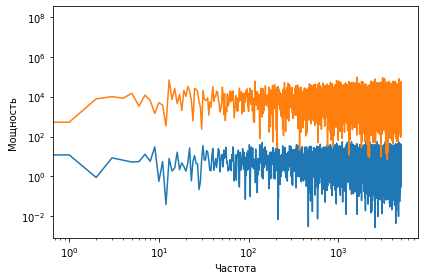
\includegraphics[scale=1]{fig/lab04/lab04_6.png}
		\caption{Сравнение спектров}
	\end{center}
\end{figure}

Видно, что при увеличении амплитуды звук больше похож на белый шум

\subsection{Упражнение 5}

В этой главе описан алгоритм генерации розового шума. Концептуально простой, но вычислительно затратный. Есть более эффективные альтернативы, такие как алгоритм Восса-Маккартни.

Используем алгоритм Voss-McCartney для генерации розового шума

\begin{lstlisting}[language=Python]
def voss(nrows, ncols=16):
    array = np.empty((nrows, ncols))
    array.fill(np.nan)
    array[0, :] = np.random.random(ncols)
    array[:, 0] = np.random.random(nrows)
    
    n = nrows
    cols = np.random.geometric(0.5, n)
    cols[cols >= ncols] = 0
    rows = np.random.randint(nrows, size=n)
    array[rows, cols] = np.random.random(n)

    df = pd.DataFrame(array)
    df.fillna(method='ffill', axis=0, inplace=True)
    total = df.sum(axis=1)

    return total.values
\end{lstlisting}

\begin{lstlisting}[language=Python]
ys = voss(11025,16)
wave = Wave(ys)
wave.plot()
\end{lstlisting}

\begin{figure}[H]
	\begin{center}
		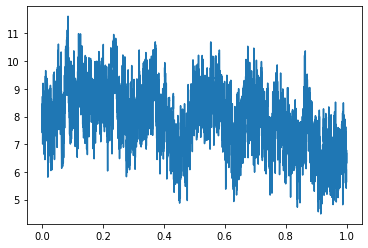
\includegraphics[scale=1]{fig/lab04/lab04_7.png}
		\caption{Сгенерированный сигнал}
	\end{center}
\end{figure}

\begin{lstlisting}[language=Python]
spectrum = wave.make_spectrum()
spectrum.hs[0] = 0
spectrum.plot_power()
decorate(xlabel='Частота',
         ylabel='Мощность',
         **loglog)
\end{lstlisting}
\begin{figure}[H]
	\begin{center}
		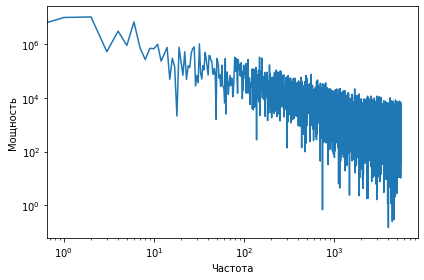
\includegraphics[scale=1]{fig/lab04/lab04_8.png}
		\caption{Спектр сигнала}
	\end{center}
\end{figure}

\begin{lstlisting}[language=Python]
spectrum.estimate_slope()[0]
\end{lstlisting}

-1.03581503502058

\noindent Видим, что в итоге был получен сигнал розового шума

\subsection{Вывод}

В данной работе были рассмотрены различные виды шумов. Шум представляет собой сигнал содержащий компоненты с различными частотами, но не имеющий гармонической структуры переодических сигналов.

\newpage

\section{Автокорреляция }
\subsection{Упражнение 1}

Оцените высоты тона вокального чирпа для нескольких времён начала сегмента.

\begin{lstlisting}[language=Python]
if not os.path.exists('28042__bcjordan__voicedownbew.wav'):
    !wget https://github.com/AllenDowney/ThinkDSP/raw/master/code/28042__bcjordan__voicedownbew.wav
from thinkdsp import read_wave
wave = read_wave('28042__bcjordan__voicedownbew.wav')
wave.normalize()
wave.make_audio()

duration = 0.01
segment1 = wave.segment(start=0.5, duration=duration)
segment1.plot()
segment2 = wave.segment(start=0.6, duration=duration)
segment2.plot()
segment3 = wave.segment(start=0.7, duration=duration)
segment3.plot()
\end{lstlisting}
\begin{figure}[H]
	\begin{center}
		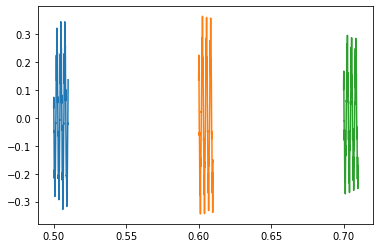
\includegraphics[scale=1]{fig/lab05/lab05_1.png}
		\caption{График сегментов}
	\end{center}
\end{figure}

Используем автокореляцию.

\begin{lstlisting}[language=Python]
lags1, corrs1 = autocorr(segment1)
plt.plot(lags1, corrs1, color='black')
decorate(xlabel='Lag', ylabel='Correlation', ylim=[-1, 1])

lags2, corrs2 = autocorr(segment2)
plt.plot(lags2, corrs2)
decorate(xlabel='Lag', ylabel='Correlation', ylim=[-1, 1])

lags3, corrs3 = autocorr(segment3)
plt.plot(lags3, corrs3, color='red')
decorate(xlabel='Lag', ylabel='Correlation', ylim=[-1, 1])
\end{lstlisting}
\begin{figure}[H]
	\begin{center}
		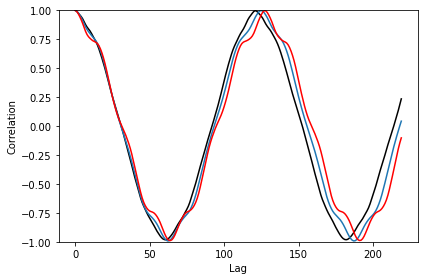
\includegraphics[scale=1]{fig/lab05/lab05_2.png}
		\caption{Автокорреляция сигналов}
	\end{center}
\end{figure}

Вычислим lag

\begin{lstlisting}[language=Python]
low = 50
high = 200
lag1 = np.array(corrs1[low:high]).argmax() + low
lag2 = np.array(corrs2[low:high]).argmax() + low
lag3 = np.array(corrs3[low:high]).argmax() + low

lag1,lag2, lag3
\end{lstlisting}
\begin{lstlisting}
(121, 125, 127)
\end{lstlisting}

Вычислим периоды

\begin{lstlisting}[language=Python]
period1 = lag1 / segment1.framerate
period2 = lag2 / segment2.framerate
period3 = lag3 / segment3.framerate
period1, period2, period3
\end{lstlisting}
\begin{lstlisting}
(0.0027437641723356007, 0.002834467120181406, 0.0028798185941043084)
\end{lstlisting}

Соответствующие периодам частоты

\begin{lstlisting}[language=Python]
frequency1 = 1 / period1
frequency2 = 1 / period2
frequency3 = 1 / period3
frequency1, frequency2, frequency3
\end{lstlisting}
\begin{lstlisting}
(364.4628099173554, 352.8, 347.244094488189)
\end{lstlisting}

\subsection{Упражнение 2}
Инкапсулировать код автокорреляции для оценки основной частоты периодического сигнала в функцию, названную estimate\_fundamental, и исользуйте её для отслеживания высоты тона записанного звука.

Используем звук из предыдущего упражнения.

\begin{lstlisting}[language=Python]
wave.make_spectrogram(2048).plot(high=4000)
\end{lstlisting}
\begin{figure}[H]
	\begin{center}
		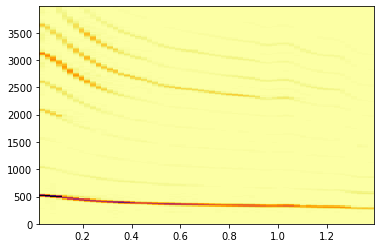
\includegraphics[scale=1]{fig/lab05/lab05_3.png}
		\caption{Спектрограмма звука}
	\end{center}
\end{figure}

Объеденим весь код из предыдущего пункта в одну функцию

\begin{lstlisting}[language=Python]
def estimate_fundamental(segment, low=50, high=200):
  lags, corrs = autocorr(segment)
  lag = np.array(corrs[low:high]).argmax() + low
  period = lag / segment.framerate
  frequency = 1 / period
  return frequency
\end{lstlisting}

\begin{lstlisting}[language=Python]
estimate_fundamental(segment1)
\end{lstlisting}
\begin{lstlisting}
364.4628099173554
\end{lstlisting}

Сделаем оценку высоты тона, применяя разделение на сегменты

\begin{lstlisting}[language=Python]
duration = wave.duration
step = 0.02
start = 0
time = []
frequencys = []
while start + step < duration:
  time.append(start + step/2)
  frequencys.append(estimate_fundamental(wave.segment(start=start,duration=step)))
  start += step
wave.make_spectrogram(2048).plot(high=900)
plt.plot(time, frequencys, color='black')
decorate(xlabel='Time (s)', ylabel='Frequency (Hz)')
\end{lstlisting}
\begin{figure}[H]
	\begin{center}
		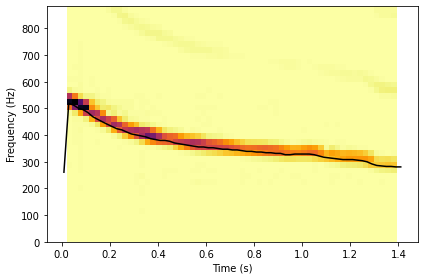
\includegraphics[scale=1]{fig/lab05/lab05_4.png}
		\caption{Результат оценки}
	\end{center}
\end{figure}

\subsection{Упражнение 3}

Вычислить автокорреляцию цен в платёжной системе Bitcoin. Оценить автокореляцию и проверить на признаки переодичности процесса.

\begin{lstlisting}[language=Python]
if not os.path.exists('market-pric.csv'):
    !wget https://github.com/Eugenepolyt/telecomunaction/raw/main/market-pric.csv

import pandas as pd
from thinkdsp import Wave

df = pd.read_csv('market-pric.csv', parse_dates=[0])
ys = df['market-price']
ts = df.index

w = Wave(ys, framerate=1)
w.plot()

\end{lstlisting}
\begin{figure}[H]
	\begin{center}
		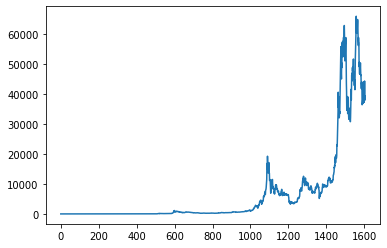
\includegraphics[scale=1]{fig/lab05/lab05_5.png}
		\caption{График цены на BitCoin}
	\end{center}
\end{figure}

Вычислим автокорреляцию:

\begin{lstlisting}[language=Python]
lags, corrs = autocorr(w)
plt.plot(lags, corrs)
decorate(xlabel='Lag',
        ylabel='Correlation')
\end{lstlisting}
\begin{figure}[H]
	\begin{center}
		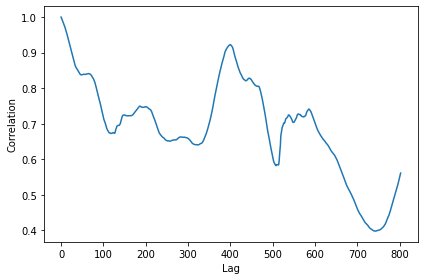
\includegraphics[scale=1]{fig/lab05/lab05_6.png}
		\caption{Автокорреляция функции цены на BitCoin}
	\end{center}
\end{figure}

По графику видно, что есть резкие спады и повышения. Процесс может напоминать переодичность.

\subsection{Упражнение 4}

В репозитории этой книги есть блокнот Jupyter под названием saxophone.ipynb, в котором исследуются автокорреляция, восприятие высоты тона и явление, называемое подавленная основная. Прочтите этот блокнот и «погоняйте» примеры. Выберите другой сегмент записи и вновь поработайте с примерами.

\begin{lstlisting}[language=Python]
if not os.path.exists('100475__iluppai__saxophone-weep.wav'):
    !wget https://github.com/AllenDowney/ThinkDSP/raw/master/code/100475__iluppai__saxophone-weep.wav
wave = read_wave('100475__iluppai__saxophone-weep.wav')
wave.normalize()
wave.make_audio()
spectrogram = wave.make_spectrogram(seg_length=1024)
spectrogram.plot(high=3000)
decorate(xlabel='Time (s)', ylabel='Frequency (Hz)')
\end{lstlisting}
\begin{figure}[H]
	\begin{center}
		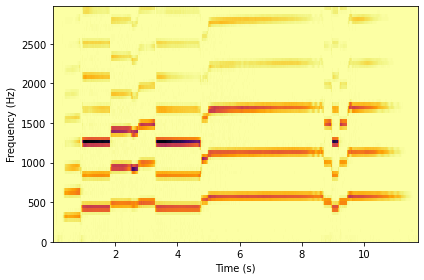
\includegraphics[scale=1]{fig/lab05/lab05_7.png}
		\caption{Спектрограмма сегмента}
	\end{center}
\end{figure}

Используем функции из блокнтота из репозитория и используем их для другого сегмента

\begin{lstlisting}[language=Python]
segment = wave.segment(start=4.0, duration=0.2)
segment.make_audio()
spectrum = segment.make_spectrum()
spectrum.plot(high=5000)
decorate(xlabel='Frequency', ylabel='Amplitude')
\end{lstlisting}

\begin{figure}[H]
	\begin{center}
		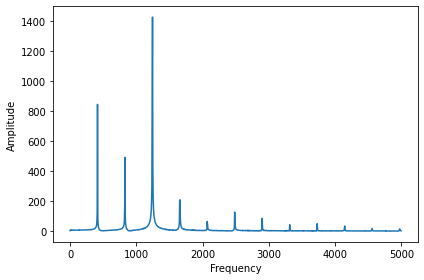
\includegraphics[scale=1]{fig/lab05/lab05_8.png}
		\caption{Спектр другого сегмента}
	\end{center}
\end{figure}

Пики в спектре находятся на 1245, 415 и 830 Гц

\begin{lstlisting}[language=Python]
spectrum.peaks()[:10]
\end{lstlisting}

\begin{lstlisting}
[(1425.371205417228, 1245.0),
 (844.1565084866448, 415.0),
 (810.3146734198679, 1240.0),
 (491.1468807713408, 830.0),
 (395.0157320768441, 1250.0),
 (285.5428668623747, 1235.0),
 (220.80813321938248, 1255.0),
 (208.75420107735613, 1660.0),
 (205.643155157793, 1655.0),
 (180.59606616391875, 1230.0)]
\end{lstlisting}

Сравним наш сегмент с треугольным сигналом

\begin{lstlisting}[language=Python]
from thinkdsp import TriangleSignal
TriangleSignal(freq=415).make_wave(duration=0.2).make_audio()
segment.make_audio()
\end{lstlisting}

У сигналов одинаковая воспринимаемая частота звука. Для понимания процесса восприятия основной частоты испольщуем АКФ.

\begin{lstlisting}[language=Python]
def autocorr2(segment):
    corrs = np.correlate(segment.ys, segment.ys, mode='same')
    N = len(corrs)
    lengths = range(N, N//2, -1)

    half = corrs[N//2:].copy()
    half /= lengths
    half /= half[0]
    return half

corrs = autocorr2(segment)
plt.plot(corrs[:500])
\end{lstlisting}

\begin{figure}[H]
	\begin{center}
		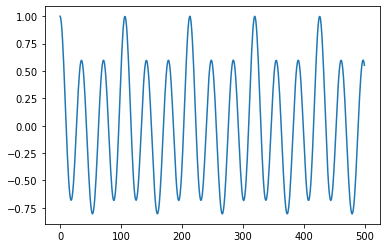
\includegraphics[scale=1]{fig/lab05/lab05_9.png}
		\caption{График после АКФ}
	\end{center}
\end{figure}

Первый пик находился возле lag 100

Найдём основную частоту при помощи написанной ранее функции.

\begin{lstlisting}[language=Python]
estimate_fundamental(segment)
\end{lstlisting}

\begin{lstlisting}
416.0377358490566
\end{lstlisting}

Воспринимаемая высота тона не изменится, если мы полностью удалим основной тон. Вот как выглядит спектр, если мы используем фильтр верхних частот, чтобы стереть основные частоты

\begin{lstlisting}[language=Python]
spectrum2 = segment.make_spectrum()
spectrum2.high_pass(600)
spectrum2.plot(high=3000)
decorate(xlabel='Frequency (Hz)', ylabel='Amplitude')
\end{lstlisting}

\begin{figure}[H]
	\begin{center}
		\includegraphics[scale=1]{fig/lab05/lab05_10.png}
		\caption{Спектр после ФНЧ}
	\end{center}
\end{figure}

Это явление называется "отсутствующим фундаментом"
Чтобы понять, почему мы слышим частоту, которой нет в сигнале, полезно взглянуть на функцию автокорреляции (ACF).

\begin{lstlisting}[language=Python]
corrs = autocorr2(segment2)
plt.plot(corrs[:500])
\end{lstlisting}

\begin{figure}[H]
	\begin{center}
		\includegraphics[scale=1]{fig/lab05/lab05_11.png}
		\caption{Полученный график}
	\end{center}
\end{figure}

\begin{lstlisting}[language=Python]
estimate_fundamental(segment)
\end{lstlisting}

\begin{lstlisting}
416.0377358490566
\end{lstlisting}

Таким образом, эти эксперименты показывают, что восприятие высоты тона основано не только на спектральном анализе, но и на чем-то вроде автокорреляции.

\subsection{Вывод}

В данной работе мы изучили корреляцию и как она влияет на сигналы, также был написан код для сигнала с "отсутствующим фунтаментом".



\newpage

\section{Дискретное косинусное преобразование }
\subsection{Упражнение 1}

Убедимся, что analyze1 требует времени пропорционально n^3, а analyze2 пропорционален n^2 c помощью команды %timeit.

\begin{lstlisting}[language=Python]
import numpy as np
PI2 = np.pi * 2
def analyze1(ys, fs, ts):
    args = np.outer(ts, fs)
    M = np.cos(PI2 * args)
    amps = np.linalg.solve(M, ys)
    return amps
def analyze2(ys, fs, ts):
    args = np.outer(ts, fs)
    M = np.cos(PI2 * args)
    amps = M.dot(ys) / 2
    return amps
\end{lstlisting}

Возьмём размеры массива как степени 2.

\begin{lstlisting}[language=Python]
ns = 2 ** np.arange(5,10)
\end{lstlisting}

\begin{lstlisting}[language=Python]
best_analyze1 = []
for n in ns:
    ts = (0.5 + np.arange(n)) / n
    freqs = (0.5 + np.arange(n)) / 2
    ys = wave.ys[:n]
    best =  %timeit -r1 -o analyze1(ys,freqs,ts)
    best_analyze1.append(best.best)
best_analyze2 = []
for n in ns:
    ts = (0.5 + np.arange(n)) / n
    freqs = (0.5 + np.arange(n)) / 2
    ys = wave.ys[:n]
    best =  %timeit -r1 -o analyze2(ys,freqs,ts)
    best_analyze2.append(best.best)
best_dct = []
for n in ns:
    ys = wave.ys[:n]
    best =  %timeit -r1 -o scipy.fftpack.dct(ys, type=3)
    best_dct.append(best.best)
plt.plot(ns, best_analyze1, label='analyze1')
plt.plot(ns, best_analyze2, label='analyze2')
plt.plot(ns, best_dct, label='fftpack.dct')
loglog = dict(xscale='log', yscale='log')
decorate(xlabel='Wave length (N)', ylabel='Time (s)', **loglog)
\end{lstlisting}

\begin{figure}[H]
	\begin{center}
		\includegraphics[scale=1]{fig/lab06/lab06_1.png}
		\caption{Время работы различных методов ДКП}
	\end{center}
\end{figure}

Не смотря на теоритическое время исполнения, время analyze1 получилсось пропорциональным  n2 .

\subsection{Упражнение 2}

Реализуем алгоритм ДКП и применим его для записи звуков или речи.

Возьмем звук пианино из первой лабораторной работы

\begin{lstlisting}[language=Python]
if not os.path.exists('jcveliz__violin-origional.wav'):
    !wget https://github.com/Eugenepolyt/telecomunaction/raw/main/jcveliz__violin-origional.wav
\end{lstlisting}

Выделим сегмент:

\begin{lstlisting}[language=Python]
segment = wave.segment(start = 1.2,duration = 0.5)
segment.normalize()
segment.make_audio()
\end{lstlisting}

DCT график для полученного сегмента

\begin{lstlisting}[language=Python]
dct = segment.make_dct()
dct.plot(high = 5000)
\end{lstlisting}


\begin{figure}[H]
	\begin{center}
		\includegraphics[scale=1]{fig/lab06/lab06_2.png}
		\caption{DCT график}
	\end{center}
\end{figure}

Следующая функция принимает dct и устанавливает все элементы ниже порога "trash" в ноль

\begin{lstlisting}[language=Python]
def compress(dct, thresh=1):
    count = 0
    for i, amp in enumerate(dct.amps):
        if np.abs(amp) < thresh:
            dct.hs[i] = 0
            count += 1
            
    n = len(dct.amps)
    print(count, n, 100 * count / n, sep='\t')
\end{lstlisting}

Применим функцию для нашего сегмента

\begin{lstlisting}[language=Python]
seg_dct = segment.make_dct()
compress(seg_dct, thresh=100)
seg_dct.plot(high=4000)
\end{lstlisting}
\begin{figure}[H]
	\begin{center}
		\includegraphics[scale=1]{fig/lab06/lab06_3.png}
		\caption{DCT после фильтрации}
	\end{center}
\end{figure}


\subsection{Управжнение 3}

В блокноте phase.ipynb взять другой сегмент звука и повторить эксперименты.

\begin{lstlisting}[language=Python]
from thinkdsp import SawtoothSignal
signal = SawtoothSignal(freq=500, offset=0)
wave.segment(start=0.02,duration=0.01).plot()
decorate(xlabel='Time (s)')
\end{lstlisting}
\begin{figure}[H]
	\begin{center}
		\includegraphics[scale=1]{fig/lab06/lab06_4.png}
		\caption{График сегмента}
	\end{center}
\end{figure}

\begin{lstlisting}[language=Python]
spectrum = wave.make_spectrum()
spectrum.plot()
decorate(xlabel='Frequency (Hz)',
         ylabel='Amplitude')
\end{lstlisting}

\begin{figure}[H]
	\begin{center}
		\includegraphics[scale=1]{fig/lab06/lab06_5.png}
		\caption{Спектр сегмента}
	\end{center}
\end{figure}

\begin{lstlisting}[language=Python]
def plot_angle(spectrum, thresh=1):
    angles = spectrum.angles
    angles[spectrum.amps < thresh] = np.nan
    plt.plot(spectrum.fs, angles, 'x')
    decorate(xlabel='Frequency (Hz)', 
             ylabel='Phase (radian)')
plot_angle(spectrum, thresh=0)
plot_angle(spectrum, thresh=1)
def plot_three(spectrum, thresh=1):
    """Plot amplitude, phase, and waveform.
    
    spectrum: Spectrum object
    thresh: threshold passed to plot_angle
    """
    plt.figure(figsize=(10, 4))
    plt.subplot(1,3,1)
    spectrum.plot()
    plt.subplot(1,3,2)
    plot_angle(spectrum, thresh=thresh)
    plt.subplot(1,3,3)
    wave = spectrum.make_wave()
    wave.unbias()
    wave.normalize()
    wave.segment(duration=0.01).plot()
    display(wave.make_audio())
\end{lstlisting}

\begin{lstlisting}[language=Python]
plot_three(spectrum)
\end{lstlisting}
\begin{figure}[H]
	\begin{center}
		\includegraphics[scale=0.66]{fig/lab06/lab06_6.png}
		\caption{Результат работы функции}
	\end{center}
\end{figure}

\begin{lstlisting}[language=Python]
def zero_angle(spectrum):
    res = spectrum.copy()
    res.hs = res.amps
    return res
spectrum2 = zero_angle(spectrum)
plot_three(spectrum2)
\end{lstlisting}
\begin{figure}[H]
	\begin{center}
		\includegraphics[scale=0.66]{fig/lab06/lab06_7.png}
		\caption{Результат работы функции}
	\end{center}
\end{figure}

\begin{lstlisting}[language=Python]
def rotate_angle(spectrum, offset):
    res = spectrum.copy()
    res.hs *= np.exp(1j * offset)
    return res
\end{lstlisting}
\begin{figure}[H]
	\begin{center}
		\includegraphics[scale=0.66]{fig/lab06/lab06_8.png}
		\caption{Результат работы функции}
	\end{center}
\end{figure}


\begin{lstlisting}[language=Python]
PI2 = np.pi * 2

def random_angle(spectrum):
    res = spectrum.copy()
    angles = np.random.uniform(0, PI2, len(spectrum))
    res.hs *= np.exp(1j * angles)
    return res
spectrum4 = random_angle(spectrum)
plot_three(spectrum4)
\end{lstlisting}
\begin{figure}[H]
	\begin{center}
		\includegraphics[scale=0.66]{fig/lab06/lab06_9.png}
		\caption{Результат работы функции}
	\end{center}
\end{figure}

Звук звучит также, как первоначальный, возьмем другой звук. 

\begin{lstlisting}[language=Python]
if not os.path.exists('120994__thirsk__120-oboe.wav'):
    !wget https://github.com/AllenDowney/ThinkDSP/raw/master/code/120994__thirsk__120-oboe.wav
from thinkdsp import read_wave
wave = read_wave('120994__thirsk__120-oboe.wav')
wave.make_audio()
segment = wave.segment(start=0.2, duration=0.5)
spectrum = segment.make_spectrum()
\end{lstlisting}

\begin{lstlisting}[language=Python]
plot_three(spectrum)
\end{lstlisting}
\begin{figure}[H]
	\begin{center}
		\includegraphics[scale=0.66]{fig/lab06/lab06_10.png}
		\caption{Результат работы функции}
	\end{center}
\end{figure}

\begin{lstlisting}[language=Python]
spectrum2 = zero_angle(spectrum)
plot_three(spectrum2, thresh=50)
\end{lstlisting}
\begin{figure}[H]
	\begin{center}
		\includegraphics[scale=0.66]{fig/lab06/lab06_11.png}
		\caption{Результат работы функции}
	\end{center}
\end{figure}

Звук стал более глухой


\begin{lstlisting}[language=Python]
spectrum3 = rotate_angle(spectrum, 1)
plot_three(spectrum3, thresh=50)
\end{lstlisting}
\begin{figure}[H]
	\begin{center}
		\includegraphics[scale=0.66]{fig/lab06/lab06_12.png}
		\caption{Результат работы функции}
	\end{center}
\end{figure}


\begin{lstlisting}[language=Python]
spectrum4 = random_angle(spectrum)
plot_three(spectrum4)
\end{lstlisting}
\begin{figure}[H]
	\begin{center}
		\includegraphics[scale=0.66]{fig/lab06/lab06_13.png}
		\caption{Результат работы функции}
	\end{center}
\end{figure}

В данном случае звук уже отличается от изначального, но не сильно. Мы не слышим особо изменения в фазовой структуре, если гармоническая структура не изменялась.

\subsection{Вывод}
В данной лабораторной работе был рассмотрен ДКП , который применяется в различных форматах сжатия музыки. С помощью ДКП были рассмотрены свойства звуков с разной структурой

\newpage

\section{Дискретное преобразование Фурье }
\subsection{Упражнение 1}

Необходимо реализовать алгоритм БПФ. Для этого разделим массив сигнала на четные и нечетные элементы и затем вычислить ДФТ для обоих групп.
Также используем лемму Дэниеолсона-Ланцоша.

Для тестирования возьмем небольшой массив сигнала

\begin{lstlisting}[language=Python]
ys = [0.8, 0.7, -0.5, 0.5]
hs = np.fft.fft(ys)
hs
\end{lstlisting}
\begin{lstlisting}
array([ 1.5+0.j ,  1.3-0.2j, -0.9+0.j ,  1.3+0.2j])
\end{lstlisting}

Применим ДФТ функцию, которая представлена в предыдущем пункте, то есть в блокноте к главе книги.

\begin{lstlisting}[language=Python]
hs2 = dft(ys)
np.sum(np.abs(hs - hs2))
\end{lstlisting}
\begin{lstlisting}
7.249538831146999e-16
\end{lstlisting}

Теперь реализуем БПФ без рекурсии при помощи разделения элементов.

\begin{lstlisting}[language=Python]
def fft(ys):
  He = dft(ys[::2])
  Ho = dft(ys[1::2])
  ns = np.arange(len(ys))
  W = np.exp(-1j * PI2 * ns / len(ys))
  return np.tile(He, 2) + W * np.tile(Ho, 2)
\end{lstlisting}

\begin{lstlisting}[language=Python]
fft(ys)
\end{lstlisting}
\begin{lstlisting}
array([ 1.5+0.j ,  1.3-0.2j, -0.9-0.j ,  1.3+0.2j])
\end{lstlisting}

Теперь реализуем вариант алгоритма с рекурсией

\begin{lstlisting}[language=Python]
def fft_rec(ys):
  if len(ys) == 1:
    return ys
  He = fft_rec(ys[::2])
  Ho = fft_rec(ys[1::2])
  ns = np.arange(len(ys))
  W = np.exp(-1j * PI2 * ns / len(ys))
  return np.tile(He, 2) + W * np.tile(Ho, 2)
\end{lstlisting}

\begin{lstlisting}[language=Python]
fft_rec(ys)
\end{lstlisting}
\begin{lstlisting}
array([ 1.5+0.j ,  1.3-0.2j, -0.9-0.j ,  1.3+0.2j])
\end{lstlisting}

\subsection{Вывод}

В данной лабораторной работе был реализован алгоритм БПФ и протестирован, алгоритм работает в точности также, как и библиотечная функция. 

\newpage

\section{Фильтрация и свертка }
\subsection{Упражнение 1}

Что случится, если при увеличении std не менять M

\begin{lstlisting}[language=Python]
slider = widgets.IntSlider(min=2, max=100, value=11)
slider2 = widgets.FloatSlider(min=0, max=20, value=2)
interact(plot_filter, M=slider, std=slider2);
\end{lstlisting}

\begin{figure}[H]
	\begin{center}
		\includegraphics[scale=1]{fig/lab08/lab08_1.png}
		\caption{Гауссово окно для фильтрации}
	\end{center}
\end{figure}

\begin{lstlisting}[language=Python]
gaussian = scipy.signal.gaussian(M=11, std=11)
gaussian /= sum(gaussian)

plt.plot(gaussian, label='Gaussian')
decorate(xlabel='Index')
\end{lstlisting}
\begin{figure}[H]
	\begin{center}
		\includegraphics[scale=0.7]{fig/lab08/lab08_2.png}
		\caption{Гауссово окно}
	\end{center}
\end{figure}

\begin{lstlisting}[language=Python]
gaussian = scipy.signal.gaussian(M=11, std=1000)
gaussian /= sum(gaussian)

plt.plot(gaussian, label='Gaussian')
decorate(xlabel='Index')
\end{lstlisting}
\begin{figure}[H]
	\begin{center}
		\includegraphics[scale=0.7]{fig/lab08/lab08_3.png}
		\caption{Гауссово окно}
	\end{center}
\end{figure}

По графикам видно что кривая стала шире а БПФ меньше.

\subsection{Упражнение 2}

Выясним что происходит с преобразованием Фурье, если меняется std.

\begin{lstlisting}[language=Python]
gaussian = scipy.signal.gaussian(M=16, std=2)
gaussian /= sum(gaussian)

plt.plot(gaussian, label='Gaussian')
decorate(xlabel='Index')
\end{lstlisting}
\begin{figure}[H]
	\begin{center}
		\includegraphics[scale=0.7]{fig/lab08/lab08_4.png}
		\caption{Гауссово окно}
	\end{center}
\end{figure}

\begin{lstlisting}[language=Python]
gaussian_fft = np.fft.fft(gaussian)
plt.plot(abs(gaussian_fft), label='Gaussian')
\end{lstlisting}
\begin{figure}[H]
	\begin{center}
		\includegraphics[scale=1]{fig/lab08/lab08_5.png}
		\caption{FTT применённое на окно}
	\end{center}
\end{figure}

Сделаем свертку отрицательных частот влево.

\begin{lstlisting}[language=Python]
gaussian_fft_rolled = np.roll(gaussian_fft, len(gaussian) // 2)
plt.plot(abs(gaussian_fft_rolled), label='Gaussian')
\end{lstlisting}
\begin{figure}[H]
	\begin{center}
		\includegraphics[scale=1]{fig/lab08/lab08_6.png}
		\caption{Результат свертки}
	\end{center}
\end{figure}

При увеличении std гауссовой кривой, преобразование Фурье становится уже.


\subsection{Упражнение 3}

Поработать с разными окнами. Какое из них лучше подходит для филтра НЧ?

Создадим сигнал длительностью 1 секунда для тестирования.

\begin{lstlisting}[language=Python]
import thinkdsp
sig = thinkdsp.TriangleSignal(freq=440)
wave = sig.make_wave(duration=1.0, framerate=44100)
wave.make_audio()
\end{lstlisting}

\begin{lstlisting}[language=Python]
sig.plot()
\end{lstlisting}

\begin{figure}[H]
	\begin{center}
		\includegraphics[scale=1]{fig/lab08/lab08_7.png}
		\caption{Пилообразный сигнал}
	\end{center}
\end{figure}

Создадим различные окна


\begin{lstlisting}[language=Python]
M = 16
std = 2

g = scipy.signal.gaussian(M,std)
br = np.bartlett(M)
bl = np.blackman(M)
hm = np.hamming(M)
hn = np.hanning(M)

array  = [gaussian,bartlett,blackman,hamming,hanning]
labels = ['gauss','barlett','blackman','hamming','hanning']

for elem, label in zip(array,labels):
  elem /= sum(elem)
  plt.plot(elem,label=label)
plt.legend()
\end{lstlisting}

\begin{figure}[H]
	\begin{center}
		\includegraphics[scale=1]{fig/lab08/lab08_8.png}
		\caption{Применение различных окон на выбранный сигнал}
	\end{center}
\end{figure}

Дополним окна нулями и выведем ДПФ:

\begin{lstlisting}[language=Python]
for elem, label in zip(array, labels):
  padded =  zero_pad(elem, len(wave))
  dft_window = np.fft.rfft(padded)
  plt.plot(abs(dft_window), label=label)
plt.legend()
\end{lstlisting}
\begin{figure}[H]
	\begin{center}
		\includegraphics[scale=1]{fig/lab08/lab08_9.png}
		\caption{Применение различных окон на выбранный сигнал}
	\end{center}
\end{figure}

Изменим маштаб.

\begin{lstlisting}[language=Python]
for elem, label in zip(array, labels):
  padded =  zero_pad(elem, len(wave))
  dft_window = np.fft.rfft(padded)
  plt.plot(abs(dft_window), label=label)
plt.legend()
decorate(yscale='log')
\end{lstlisting}
\begin{figure}[H]
	\begin{center}
		\includegraphics[scale=1]{fig/lab08/lab08_10.png}
		\caption{Логорифмический масштаб}
	\end{center}
\end{figure}

Кажется, что хэнинг лучше всего подоёдет для фильтрации НЧ.

\subsection{Вывод}

В данной работе были рассмотренны операции фильстрации , сглаживания и свертки. Каждая функция может быть полезной для какой-либо определенной задачи, сглаживание, например, удаляет быстрые изменения сигнала для выявления общих особенностей.

\newpage

\section{Дифференциация и интеграция }
\subsection{Упражнение 1}

Создайте треугольный сигнал и напечатайте его. Примените diff к сигналу и напечатайте результат. Вычислите спектр треугольного сигнала, примените differentiate и напечатайте результат. Преобразуйте спектр обратно в сигнал и напечатайте его. Есть ли различия в воздействии diff и differentiate на этот сигнал?

\begin{lstlisting}[language=Python]
from thinkdsp import TriangleSignal

wave = TriangleSignal(freq=440).make_wave(duration=0.01, framerate=44100)
wave.plot()
decorate(xlabel='Time (s)')
\end{lstlisting}
\begin{figure}[H]
	\begin{center}
		\includegraphics[scale=1]{fig/lab09/lab09_1.png}
		\caption{График треугольного сигнала}
	\end{center}
\end{figure}

\begin{lstlisting}[language=Python]
diff_wave = wave.diff()
diff_wave.plot()
decorate(xlabel='Time (s)')
\end{lstlisting}
\begin{figure}[H]
	\begin{center}
		\includegraphics[scale=1]{fig/lab09/lab09_2.png}
		\caption{Сигнал после применения diff}
	\end{center}
\end{figure}

Получился прямоугольны сигнал с такой же частотой

\begin{lstlisting}[language=Python]
differentiate_wave = wave.make_spectrum().differentiate().make_wave()
differentiate_wave.plot()
decorate(xlabel='Time (s)')
\end{lstlisting}
\begin{figure}[H]
	\begin{center}
		\includegraphics[scale=1]{fig/lab09/lab09_3.png}
		\caption{Сигнал после применения differentiate}
	\end{center}
\end{figure}

Вначале и в конце шум, вероятнее всего это связано c тем, что невозможно вычислить производную.

\subsection{Упражнение 2}

Создайте прямоугольный сигнал и напечатайте его. Примените cumsum и напечатайте результат. Вычислите спектр прямогоульного сигнала, примените integrate и напечатайте результат. Преобразуйте спектр обратно в сигнал и напечайте его. Есть различия в воздействии cumsum и integrate на этот сигнал?

Изучим влияние cumsum и integrate на прямоугольный сигнал.

\begin{lstlisting}[language=Python]
from thinkdsp import SquareSignal

wave = SquareSignal(freq=100).make_wave(duration=0.1, framerate=44100)
wave.plot()
decorate(xlabel='Time (s)')
\end{lstlisting}
\begin{figure}[H]
	\begin{center}
		\includegraphics[scale=1]{fig/lab09/lab09_4.png}
		\caption{Рассматриваемый сигнал}
	\end{center}
\end{figure}

Применим cumsum:

\begin{lstlisting}[language=Python]
cumsum_wave = wave.cumsum()
cumsum_wave.plot()
decorate(xlabel='Time (s)')
\end{lstlisting}
\begin{figure}[H]
	\begin{center}
		\includegraphics[scale=1]{fig/lab09/lab09_5.png}
		\caption{Рассматриваемый сигнал после применения cumsum}
	\end{center}
\end{figure}

Получился треугольный сигнал

Теперь интеграл спектра:

\begin{lstlisting}[language=Python]
int_spec = wave.make_spectrum().integrate()
int_spec.hs[0] = 0
int_wave = int_spec.make_wave()
int_wave.plot()
decorate(xlabel='Time (s)')
\end{lstlisting}
\begin{figure}[H]
	\begin{center}
		\includegraphics[scale=1]{fig/lab09/lab09_6.png}
		\caption{Рассматриваемый сигнал после применения integrate}
	\end{center}
\end{figure}

Спектральный интеграл также получлся треугольным, однако с другой амплитудой

\subsection{Упражнение 3}

Создайте пилообразный сигнал, вычислите его спектр, а затем дважды примените integrate. Напечатйте результирующий сигнал и его спектр. Какова математическая форма сигнала? Почему он напоминает синусойду?

Изучим влияние двойного интегрирования на пилообразный сигнал.

\begin{lstlisting}[language=Python]
from thinkdsp import SawtoothSignal

wave = SawtoothSignal(freq=100).make_wave(duration=0.1, framerate=44100)
wave.plot()
decorate(xlabel='Time (s)')
\end{lstlisting}
\begin{figure}[H]
	\begin{center}
		\includegraphics[scale=1]{fig/lab09/lab09_7.png}
		\caption{Пилообразный сигнал}
	\end{center}
\end{figure}

\begin{lstlisting}[language=Python]
spectrum = wave.make_spectrum().integrate().integrate()
spectrum.hs[0] = 0
wave1 = spectrum.make_wave()
wave1.plot()
decorate(xlabel='Time (s)')
\end{lstlisting}
\begin{figure}[H]
	\begin{center}
		\includegraphics[scale=1]{fig/lab09/lab09_8.png}
		\caption{Изменённый сигнал}
	\end{center}
\end{figure}

Сигнал напоминает синусойду, это связано с фильтрацией низких частот кроме основной.

\begin{lstlisting}[language=Python]
wave.make_spectrum().plot(high=1000)
\end{lstlisting}
\begin{figure}[H]
	\begin{center}
		\includegraphics[scale=1]{fig/lab09/lab09_9.png}
		\caption{Спектр исходного сигнала}
	\end{center}
\end{figure}

\begin{lstlisting}[language=Python]
wave1.make_spectrum().plot(high=1000)
\end{lstlisting}
\begin{figure}[H]
	\begin{center}
		\includegraphics[scale=1]{fig/lab09/lab09_10.png}
		\caption{Спектр нового сигнала}
	\end{center}
\end{figure}


\subsection{Упражнение 4}

Создайте CubicSignal, определённый в thinkdsp. Вычислите вторую разность, дважды применив diff. Как выглядит результат? Вычислите вторую разность, дважды применив differentiate к спектру. Похожи ли результаты? Распечатйте фильтры, соответсвующие второй разнице и второй производной. Сравните их.

Изучим влияние второй разности и второй производной на CubicSignal сигнале.

\begin{lstlisting}[language=Python]
from thinkdsp import CubicSignal
w = CubicSignal(freq=0.0005).make_wave(duration=10000, framerate=1)
w.plot()
\end{lstlisting}
\begin{figure}[H]
	\begin{center}
		\includegraphics[scale=1]{fig/lab09/lab09_11.png}
		\caption{Кубический сигнал}
	\end{center}
\end{figure}

Первая разность это параболы

\begin{lstlisting}[language=Python]
first = w.diff()
first.plot()
\end{lstlisting}
\begin{figure}[H]
	\begin{center}
		\includegraphics[scale=1]{fig/lab09/lab09_12.png}
		\caption{Первая разность}
	\end{center}
\end{figure}

Вторая разность это пилообразный сигнал.

\begin{lstlisting}[language=Python]
second = first.diff()
second.plot()
\end{lstlisting}
\begin{figure}[H]
	\begin{center}
		\includegraphics[scale=1]{fig/lab09/lab09_13.png}
		\caption{Вторая разность}
	\end{center}
\end{figure}

Сделаем двойное дифферинцирование.

\begin{lstlisting}[language=Python]
spec = w.make_spectrum().differentiate().differentiate()
third = spec.make_wave()
third.plot()
\end{lstlisting}
\begin{figure}[H]
	\begin{center}
		\includegraphics[scale=1]{fig/lab09/lab09_14.png}
		\caption{Полученный сигнал со звоном}
	\end{center}
\end{figure}

В связи с тем что производная не определена в некоторых точках, на графике присутствует звон, используем фильтры:

\begin{lstlisting}[language=Python]
from thinkdsp import zero_pad
from thinkdsp import Wave

diff_window = np.array([-1.0, 2.0, -1.0])
padded = zero_pad(diff_window, len(wave))
diff_wave = Wave(padded, framerate=wave.framerate)
diff_filter = diff_wave.make_spectrum()
diff_filter.plot()
decorate(xlabel='Frequency (Hz)', ylabel='Amplitude ratio')
\end{lstlisting}

\begin{figure}[H]
	\begin{center}
		\includegraphics[scale=1]{fig/lab09/lab09_15.png}
		\caption{Полученные фильтры}
	\end{center}
\end{figure}

Для второй производной можно найти соответствующий фильтр, рассчитав фильтр первой прозводной и возведя его в квадрат.
\begin{lstlisting}[language=Python]
deriv_filter = w.make_spectrum()
deriv_filter.hs = (2 * np.pi * 1j * deriv_filter.fs)**2
deriv_filter.plot()
\end{lstlisting}

\begin{figure}[H]
	\begin{center}
		\includegraphics[scale=1]{fig/lab09/lab09_16.png}
		\caption{Полученные фильтры}
	\end{center}
\end{figure}


\subsection{Вывод}

В данной работе были рассмотрены соотношения между окнами во временной области и фильтрами в частотной. Также рассмотрели конечные разности, cumsum - накапливающие суммы с апроксимирующим интегрированием.

\newpage

\section{Сигналы и системы }
\subsection{Упражнение 1}

Измените пример в chap10.ipynb и убедитесь, что дополнение нулями устраняет лишнюю ноту в начале фрагмента:

Устраним проблему с лишней нотой путем добавления нулей в конец сигнала.

\begin{lstlisting}[language=Python]
from thinkdsp import read_wave

response = read_wave('180960__kleeb__gunshot.wav')
start = 0.12
response = response.segment(start=start)
response.shift(-start)
response.normalize()
response.plot()
decorate(xlabel='Time (s)')
\end{lstlisting}
\begin{figure}[H]
	\begin{center}
		\includegraphics[scale=1]{fig/lab10/lab10_1.png}
		\caption{Сигнал}
	\end{center}
\end{figure}

\begin{lstlisting}[language=Python]
spec = response.make_spectrum()
spec.plot()
decorate(xlabel='Frequency (Hz)', ylabel='Amplitude')
\end{lstlisting}
\begin{figure}[H]
	\begin{center}
		\includegraphics[scale=1]{fig/lab10/lab10_2.png}
		\caption{Спектр сигнала}
	\end{center}
\end{figure}

Теперь перейдём к самой записе:

\begin{lstlisting}[language=Python]
violin = read_wave('92002__jcveliz__violin-origional.wav')
start = 0.11
violin = violin.segment(start=start)
violin.shift(-start)
violin.truncate(len(response))
violin.normalize()
violin.plot()
decorate(xlabel='Time (s)')
\end{lstlisting}
\begin{figure}[H]
	\begin{center}
		\includegraphics[scale=1]{fig/lab10/lab10_3.png}
		\caption{График сигнала}
	\end{center}
\end{figure}

\begin{lstlisting}[language=Python]
spec2 = violin.make_spectrum()
\end{lstlisting}

Теперь умножим ДПФ сигнала на передаточную функцию и преобразуем обратно в волну.

\begin{lstlisting}[language=Python]
wave = (spec * spec2).make_wave()
wave.normalize()
wave.plot()
\end{lstlisting}
\begin{figure}[H]
	\begin{center}
		\includegraphics[scale=1]{fig/lab10/lab10_4.png}
		\caption{График получившегося сигнала}
	\end{center}
\end{figure}

Проблему удалось решить.

\subsection{Упражнение 2}

Необходимо смоделировать двумя способами звучание записи в том пространстве, где была измерена импульсная харпактеристика, как свёрткой самой записи с импульсной характеристикой, так и умножением ДПФ записи на вычисленный фильтр, соотвествующий импульсной характеристики. Характеристику возьмем из учебника.


\begin{lstlisting}[language=Python]
if not os.path.exists('stalbans_a_mono.wav'):
    !wget https://github.com/AllenDowney/ThinkDSP/raw/master/code/stalbans_a_mono.wav

response = read_wave('stalbans_a_mono.wav')

start = 0
duration = 5
response = response.segment(duration=duration)
response.shift(-start)
response.normalize()
response.plot()
decorate(xlabel='Time (s)')
decorate(xlabel='Time (s)')
\end{lstlisting}
\begin{figure}[H]
	\begin{center}
		\includegraphics[scale=1]{fig/lab10/lab10_5.png}
		\caption{График загруженного сигнала}
	\end{center}
\end{figure}

ДПФ:

\begin{lstlisting}[language=Python]
transfer = response.make_spectrum()
transfer.plot()
\end{lstlisting}
\begin{figure}[H]
	\begin{center}
		\includegraphics[scale=1]{fig/lab10/lab10_6.png}
		\caption{ДПФ импульсной характеристики}
	\end{center}
\end{figure}

Промоделируем запись в пространстве, будем также использовать звук из учебника - скрипку

\begin{lstlisting}[language=Python]
wave = read_wave('92002__jcveliz__violin-origional.wav')
start = 0.0
wave = wave.segment(start=start)
wave.shift(-start)
wave.truncate(len(response))
wave.normalize()
wave.plot()
\end{lstlisting}
\begin{figure}[H]
	\begin{center}
		\includegraphics[scale=1]{fig/lab10/lab10_7.png}
		\caption{Сигнал звука скрипки}
	\end{center}
\end{figure}


\begin{lstlisting}[language=Python]
spectrum = wave.make_spectrum()
len(spectrum.hs), len(transfer.hs)
\end{lstlisting}
\begin{lstlisting}
(110251, 110251)
\end{lstlisting}

\begin{lstlisting}[language=Python]
spectrum.fs, transfer.fs
\end{lstlisting}
\begin{lstlisting}
(array([0.00000e+00, 2.00000e-01, 4.00000e-01, ..., 2.20496e+04,
        2.20498e+04, 2.20500e+04]),
 array([0.00000e+00, 2.00000e-01, 4.00000e-01, ..., 2.20496e+04,
        2.20498e+04, 2.20500e+04]))
\end{lstlisting}

Используем свертку.

\begin{lstlisting}[language=Python]
con = wave.convolve(response)
con.normalize()
con.make_audio()
\end{lstlisting}

Используем умножение:
\begin{lstlisting}[language=Python]
result = (spectrum * transfer).make_wave()
result.normalize()
result.plot()
\end{lstlisting}

\begin{figure}[H]
	\begin{center}
		\includegraphics[scale=1]{fig/lab10/lab10_7.png}
		\caption{Полученный график}
	\end{center}
\end{figure}

\subsection{Вывод}

В данной работе мы рассмотрели основные позиции из теории сигналов и систем, например музыкальную акустику. При описании линейных стационарных систем используется теорема о свёртке.

\newpage

\section{Модуляция и сэмплирование }
\subsection{Упражнение 1}

При взятии выборок из сигнала при слишком низкой чистоте кадров составляющие, большие частоты заворота дадут биения. В таком случаее эти компоненты не отфильтруешь, посколько они неотличимы от более низких частот. Полезно отфильтровать эти частоты до выборки: фильтр НЧ, используемый для этой цели, называется фильтром сглаживания. Вернитесь к примеру "Соло на барабане", примените фильтр НЧ до выборки, а затем, опять с помощью фильтра НЧ, удалите спектральные копии, вызванные выборкой. Результат должен быть идентицент отфильтрованному сигналу.

Возьмем звук барабанов, применим фильтр НЧ до выборки, а затем, опять с помощью фильтра НЧ удалим спектральные копии, вызванные выборкой.

\begin{lstlisting}[language=Python]
wave = read_wave('263868__kevcio__amen-break-a-160-bpm.wav')
wave.plot()
\end{lstlisting}
\begin{figure}[H]
	\begin{center}
		\includegraphics[scale=1]{fig/lab11/lab11_1.png}
		\caption{График звука барабанов}
	\end{center}
\end{figure}

\begin{lstlisting}[language=Python]
spectrum = wave.make_spectrum(full=True)
spectrum.plot()
\end{lstlisting}
\begin{figure}[H]
	\begin{center}
		\includegraphics[scale=1]{fig/lab11/lab11_2.png}
		\caption{Спектр сигнала}
	\end{center}
\end{figure}

Применим фильтр низких частот:

\begin{lstlisting}[language=Python]
factor = 3
framerate = wave.framerate / factor
cutoff = framerate / 2 - 1

spectrum.low_pass(cutoff)
spectrum.plot()
\end{lstlisting}
\begin{figure}[H]
	\begin{center}
		\includegraphics[scale=1]{fig/lab11/lab11_3.png}
		\caption{Отфильтрованный сигнал}
	\end{center}
\end{figure}

Применим функцию из учебника, которая имитирует процесс выборки.


\begin{lstlisting}[language=Python]
sampled = sample(filtered, factor)
sampled.make_audio()

sampled_spectrum = sampled.make_spectrum(full=True)
sampled_spectrum.plot()
\end{lstlisting}
\begin{figure}[H]
	\begin{center}
		\includegraphics[scale=1]{fig/lab11/lab11_4.png}
		\caption{Получившийся спектр}
	\end{center}
\end{figure}


Теперь удалим спектральные копии:
\begin{lstlisting}[language=Python]
sampled_spectrum.low_pass(cutoff)
sampled_spectrum.plot()
\end{lstlisting}
\begin{figure}[H]
	\begin{center}
		\includegraphics[scale=1]{fig/lab11/lab11_5.png}
		\caption{Результат избавления от копий}
	\end{center}
\end{figure}

Сравним звуки

\begin{lstlisting}[language=Python]
spectrum.make_wave().make_audio()

interpolated = sampled_spectrum.make_wave()
interpolated.make_audio()

spectrum.plot()
sampled_spectrum.plot()
\end{lstlisting}

\begin{figure}[H]
	\begin{center}
		\includegraphics[scale=1]{fig/lab11/lab11_6.png}
		\caption{Сравнение спектров}
	\end{center}
\end{figure}

Звуки отличаются , увеличим амлитуду в три раза:

\begin{lstlisting}[language=Python]
sampled_spectrum.scale(factor)
sampled_spectrum.plot()
spectrum.plot()
\end{lstlisting}
\begin{figure}[H]
	\begin{center}
		\includegraphics[scale=1]{fig/lab11/lab11_7.png}
		\caption{Сравнение спектров}
	\end{center}
\end{figure}

В итоге разница между интерполированной волной и фильтрованной волной есть, но она едва заметная.

\subsection{Вывод}

В данной работе были проверены свойства выборок и прояснены биения и заворот частот.

\newpage

\section{FSK}
\subsection{Описание работы FSK}

Frequency Shift Key - вид модуляции, при которой скачкообразно изменяется частота несущего сигнала в зависимости от значений символов информационной последовательности. Частотная модуляция весьма помехоустойчива, так как помехи искажают в основном амплитуду, а не частоту сигнала.

Для модулирования и тестирования данного процесса, необходимо построить следующую схему в графическом интерфейсе GNU Radio
    
    \begin{landscape}
	\begin{figure}[H]
		\centering
		\includegraphics[width=25.5cm]{fig/lab12/lab12_1.png}
		\caption{Схема FSK}
		\label{pic:fsk_scheme} % название для ссылок внутри кода
	\end{figure}
\end{landscape}

В данной схеме используются следующие блоки:

\begin{itemize}
	\item Frequency Xlating FIR Filter - Этот блок выполняет частотный перевод сигнала, а также понижает разрешение сигнала, запуская на нем децимирующий FIR-фильтр.
	\item Simple Squelch - Простой блок шумоподавления на основе средней мощности сигнала и порога в дБ.
	\item Quadrature Demod - Этот блок вычисляет произведение одновыборочного отложенного и сопряженного входного сигнала и нераскрытого сигнала, а затем вычисляет аргумент (также известный как угол, в радианах) результирующего комплексного числа.
	\item Binary Slicer - Нарезает числа с плавающей запятой, производя 1-битный вывод. Положительный ввод производит двоичную 1, а отрицательный ввод производит двоичный ноль. 
	\item QT GUI Sink - Выводы необходимой инфомрации в графическом интерфейсе.
    \item Options - Этот блок устанавливает некоторые общие параметры графа потоков. Такие как название проекта, авторство и другие. 
	\item Variable - Этот блок сопоставляет значение с уникальной переменной. Есть возможность использования переменной в другом блоке, благодаря идентификатору (id) блока переменных. 
	\item Multiply Const - Умножает входной поток на скалярную или векторную константу.
	\item Add Const - Прибавляет к входному потоку скалярную или векторную константу.
	\item QT GUI Range - Этот блок создает переменную с выбором виджетов. Переменной может быть присвоено значение по умолчанию, и ее значение может быть изменено во время выполнения в указанном диапазоне.
	\item Random Source - Генератор случайных чисел.
	\item Unpack K bits - Преобразует байт с k релевантных битов в k выходных байтов с 1 битом каждый.
	\item Repeat - Количество раз для повторения входных данных, выступающих в качестве коэффициента интерполяции.
	\item Throttle - Этот блок служит для того, чтобы дросселировать поток так, чтобы средняя скорость не превышала удельную скорость.
	\item Uchar To Float - Преобразует unsigned chars в поток float.
	\item Virtual Sink - Служит для сохранения потока в вектор.
	\item Virtual Source - Работает в паре с Virtual Sink блоком. Источник данных, который передаёт элементы на основе входного вектора. 
	\item VCO - Генератор с регулируемым напряжением. Создает синусоиду частоты на основе амплитуды входного сигнала.
\end{itemize}

В данном примере используется скорость передачи данных для радиотелетипа Baudot, для данного типа битовое время составляет 22 миллисекунды, поэтому скорость передачи данных установлена на 1/0,022, что дает 45,4545. Коэффициент повторения (int)(samp\_rate*0,022). Для этого флоуграфа блок VCO генерирует сигналы 2295 Гц (отметка = 1) и 2125 Гц (отметка = 0). Расчеты для этого следующие:
\begin{itemize}
\item При выборе полной шкалы частоты 2500 Гц (vco\_max) для входа +1 чувствительность VCO = (2 * math.pi * 2500 / 1) = 15708. Можно использовать любую частоту выше 2295 Гц. 2500 Гц — хорошее круглое число. 
\item Глядя на вывод виртуального источника «xmt\_data», Mark = +1.0 и Space = 0.0. 
\item Диапазон частон 2125 Гц создается при помощи vco\_offset = (2125 / 2500) = 0,850 + (0,0 * 0,068)
\item Частота отметки 2295 Гц создается вектором inp\_amp = (1,0 * 0,068) + vco\_offset = 0,918, что равно (2295/2500). Параметр отводов частотного Xlating FIR Filter равен 'firdes.low\_pass(1.0,samp\_rate,1000,400)'.
\end{itemize}

Cлучайный источник (Random Source) генерирует байтовые значения от 0 до 255. Далее при помощи блока Unpack K Bits распаковывает каждый бит входных данных в виде отдельного байта со значением в младшем разряде. Для ограничения потока используется Throttle блок.

На стороне приема, Frequency Xlating FIR Filter блок смещает принимаемый сигнал так, чтобы он был сосредоточен вокруг центральной частоты - между частотами Mark и Space. Блок Quadrature Demod выдает сигнал, который является положительным для входных частот выше нуля и отрицательным для частот ниже нуля. Этот сигнал подается в блок Binary Slicer, выходные данные представляют собой байт 1 или 0, что и является полученной информацией.

\subsection{Тестирование}

    \begin{figure}[H]
	\begin{center}
		\includegraphics[scale=0.4]{fig/lab12/lab12_2.png}
		\caption{Модуляция без задержки и шума}
		\label{pic:e1} % название для ссылок внутри кода
	\end{center}
\end{figure}

На графике можно видеть 3 сигнала разного цвета. Зеленный показывает данные которые были переданы передатчиком. Синий - это данные полученные приемником. А красный отвечает за разницу между зеленым и синим. Красный сигнал должен быть равен нулю, это сигнализирует о том, что данные передаются верно, однако на диаграмме сверху видно, что это не так и выходит так, что полученная информация различается от той, которую передавали. Принятый сигнал находится на некоторое количество бит позади, потому что цепочка передатчика и приемника имеет много блоков и фильтров, которые задерживают сигнал. Для того чтобы это исправить необходимо сделать задержку между приемом и передачей данных, что и обеспечивает блок Delay. Правильном задержкой является 145. 

    \begin{figure}[H]
	\begin{center}
		\includegraphics[scale=0.3]{fig/lab12/lab12_3.png}
		\caption{Модуляция с правильной задержкой}
		\label{pic:e2} % название для ссылок внутри кода
	\end{center}
\end{figure}

Теперь как можно заметить все хорошо и данные передаются и получаются корректно. 

\subsection{Вывод}
В данной лабораторной работе был рассмотрен один из способов модуляции. При помощи GNU Radio была создана необходимая модель и протестирована. 
    
\newpage

\addcontentsline{toc}{section}{Заключение}

% Не редактируем: Страница библиографии (формируется автоматически из книжек, указанных в refs.bib и пометок \cite{имя_источника} в тексте)
\newpage
\printbibliography[title=Перечень использованных источников]
\addcontentsline{toc}{section}{Перечень использованных источников}
\end{document}
